\documentclass[12pt]{article}
\textheight=24.5cm \textwidth=16.5cm
\parskip = 0.165cm
\renewcommand\baselinestretch{1.2}
\topmargin=-2cm \oddsidemargin=0cm \evensidemargin=0cm

\usepackage{amsfonts}
\usepackage{amsmath}
\usepackage{amsthm}
\usepackage{amssymb}
\usepackage{amscd}
\usepackage{mathrsfs}
\usepackage{latexsym}
\usepackage[round, sort]{natbib}
\usepackage[colorlinks=true,linkcolor=blue,anchorcolor=black,citecolor=blue,urlcolor=black]{hyperref}
\usepackage{color}
\usepackage{xcolor}
\usepackage{array}
\usepackage{booktabs}
\usepackage{multirow}
\usepackage{colortbl}
\usepackage[ruled, linesnumbered]{algorithm2e}
\usepackage{enumerate}
\usepackage{float}
\usepackage[section]{placeins}
\usepackage{indentfirst}
\usepackage{CJKutf8}
\usepackage{tikz}
\usetikzlibrary{arrows.meta, positioning, decorations.pathreplacing}
\usepackage{pgfplots}
\pgfplotsset{compat=1.18}
\definecolor{apxblue}{RGB}{0,114,178}
\definecolor{nehred}{RGB}{213,94,0}
\definecolor{gagreen}{RGB}{0,158,115}

\allowdisplaybreaks

\newtheorem{theorem}{Theorem}[section]
\newtheorem{cor}{Corollary}[section]
\newtheorem{lemma}{Lemma}[section]
\newtheorem{rem}{Remark}[section]
\newtheorem{definition}{Definition}[section]
\newtheorem{obs}{Observation}
\newtheorem{proposition}[theorem]{Proposition}
\newtheorem{exam}{Example}[section]

% Figures and tables are numbered sequentially over the whole paper as
% "Figure 1", "Table 1", ... , independently of the section they appear
% in.  The figures of Sections 2 to 5 are drawn with the number of the
% figure inside the picture rather than captioned below it, so their blocks
% step the counter by hand; the counter must therefore not be reset at a
% section break.
\renewcommand{\thefigure}{\arabic{figure}}
\renewcommand{\thetable}{\arabic{table}}

% The tables of the experiments share one row spacing and one width, so that
% they read as one set.  Every one of them is opened with \resultstable and
% drawn on a tabular* of \resultstabwidth, whose columns are then spread over
% the whole width: the natural width of a table never has to match that of its
% neighbours.  The four comparison tables carry two columns per method and a
% pair of figures in every one of them, which is more than any of the others
% has to hold; they are therefore set one size down, with a narrower column
% separation, and the width below leaves them the room that the pair needs.
\newlength{\resultstabwidth}
\setlength{\resultstabwidth}{16.2cm}
\newcommand{\resultstable}{%
    \centering
    \footnotesize
    \setlength{\tabcolsep}{4pt}%
    \renewcommand{\arraystretch}{1.15}}

\setcounter{topnumber}{4}
\setcounter{bottomnumber}{3}
\setcounter{totalnumber}{6}
\renewcommand{\floatpagefraction}{0.9}
\renewcommand{\topfraction}{1.0}
\renewcommand{\bottomfraction}{0.6}
\renewcommand{\textfraction}{0.05}

% A barrier is placed at every section heading, so that no table or figure of
% one section is carried into the next.  The subsections are left without one:
% the tables of Section 6 are tall and stand two and three to a subsection, and
% with a barrier at the heading of each of them the text that follows a run of
% floats cannot start until the run has been laid out, which is what leaves the
% foot of the pages the tables land on empty.
\let\origsection\section
\renewcommand{\section}{\FloatBarrier\origsection}

% Tables and figures are cited with \cref / \Cref, so that the whole
% "Table 2" / "Figure 4" is one hyperlink rather than only its number,
% and so that plurals and ranges ("Tables 4 to 6") come out right.
% Loaded last: \cref has to see the counters and \newtheorem above.
\usepackage[nameinlink]{cleveref}

% Equations keep their bare "(1)" form, as \eqref produced, rather than
% cleveref's default "eq. (1)".
\crefname{equation}{}{}

% The examples are cited as "Example 4.1", like the theorems and lemmas
% above them, rather than in cleveref's fallback form.
\crefname{exam}{Example}{Examples}

\title{\LARGE\bf $F2 \parallel W C_{\max}$ Structural Properties and Dynamic Programming}
\author{Author One$^{a,}$\footnote{Corresponding author. E-mail address: author@email.com}, Author Two$^{b}$\\
{\small $^{a}$Institution One, Location, Country}\\
{\small $^{b}$Institution Two, Location, Country}\\}
\date{}

\begin{document}
\begin{sloppypar}

\maketitle

\begin{abstract}
    Minimizing the maximum weighted completion time in a two-machine flow shop models a line
    in which a few high-priority orders pace the shop. The problem is strongly NP-hard, and we
    give a mixed integer programming formulation for it. We show that an optimal schedule
    preserves the permutation property and has a block structure: one block per distinct
    weight, Johnson's order within each block, and the blocks in non-increasing weight order.
    On this structure we build three methods: a dynamic program that prunes dominated states
    and runs in $O(nKV^{3K-3})$ time, where $K$ is the number of distinct weights and $V$ the
    total processing time; a 2-approximation in $O(n\log n)$ time; and a fully polynomial-time
    approximation scheme that attains a $(1+\varepsilon)$ guarantee for a constant number of
    weights. For large instances we develop an adapted NEH heuristic and a genetic algorithm.
    In a study with twenty instances per configuration, the model settles all $440$ small
    instances, and at $K=2$ the dynamic program certifies the optimum up to eighty jobs on both
    ranges and to a hundred on the narrower one; what stops it is cost, not correctness. The
    2-approximation stays within $3.5$ per cent of the optimum on average and within $1.8$ per
    cent of the lower bound, NEH within $2.5$ and $4.4$, and the genetic algorithm, the
    weakest on small instances, is the only method whose gap falls as the instance grows,
    passing both rules beyond about $260$ jobs.
\end{abstract}

\noindent \textbf{Keywords:} Flow shop; Dynamic programming; Approximation algorithms; 

\section{Introduction}
\label{sec:intro}

The two-machine flow shop is one of the best known models in scheduling. Its structure is
that of a plant whose jobs are machined on one machine and finished on another: metal parts
are cut and then coated, a casting is rolled after it is poured, a web is printed and then
bound. A job must leave the first stage before it can enter the second, and each stage carries
one job at a time. Johnson settled the sequencing decision for this model as early as 1954
\citep{johnson1954optimal}, and the two-stage structure has remained a standard subject of
sequencing theory, with its variants and solution methods reviewed in
\citep{pinedo2022scheduling}.

The criterion of this paper is the maximum weighted completion time, also called the weighted
makespan. It charges each job the product of its weight and its completion time and takes the
largest of those products: where the makespan asks when the shop falls idle, the weighted
makespan asks which job is left waiting and what that wait costs. The weight belongs to the
order rather than to the plant as a whole, and in a plant it is rarely a continuum. A
contractual penalty for lateness, the capital tied up in work in process and the priority a
large customer has bought are three classes rather than a spectrum, and the most costly order
is the one carrying the largest of them.

Much the same structure appears outside the factory. A system that serves large language model
agents handles every step of a task in two phases: the step is reasoned about in the chain of
thought \citep{wei2022chain}, and only then acted upon, by calling a tool or running code, in
the chain of execution \citep{yao2023react}. A step is a job, the reasoning is the first
machine and the acting is the second. A step cannot be acted upon before it has been reasoned
about, each phase serves one step at a time, and the time a step spends in a phase is its
processing time on that machine. The two phases draw on different resources, the model for the
reasoning and the tool, the interpreter or the index for the acting, and the phases of
different steps run alongside each other, so that when a step finishes is settled by the phase
it is in and by the time the steps ahead of it have kept the resource it waits for. The steps
are not equal: one bought by a paid tier, or one whose failure is costly, weighs more than the
rest, and that cost is the weight of the job.

Two features of this environment are not a choice of convenience. The two stages stand in
series because a step has to be reasoned about before it is acted upon, and merging them would
erase the overlap that makes the order of the steps matter at all: reasoning and acting consume
different resources, and a step that waits for its tool leaves the model free for the next one.
The criterion is a maximum rather than an average for the same reason, since what decides
whether the service is acceptable is the step that matters most. On a single machine that step
would not be a property of the schedule: its completion time would be settled by its position
in the sequence, no earlier stage being there whose delay it could inherit. Two stages in
series are what make the completion time of the decisive step depend on the whole schedule.

In scheduling theory the criterion has been studied in several machine environments.
Maximum-type criteria have a classical foundation: Lawler's backward rule minimizes, on a single
machine, the maximum of arbitrary nondecreasing cost functions in quadratic time
\citep{lawler1973optimal}, and weighted completion times are read as a maximum rather than a sum
within that framework. In the online setting, where jobs are revealed over time, best-possible
algorithms are known for the same criterion on one machine \citep{li2015best}, and a machine
carrying one restricted rate-modifying activity has been treated for it as well
\citep{zuo2026single}. On identical parallel
machines, randomized approximation schemes have been developed for the weighted makespan
\citep{sun2024randomized}, and the criterion has been combined with the decision of which
orders to accept \citep{lu2025order}. Maximum-type criteria appear in other forms as well, such
as the maximum earliness/tardiness cost of a single machine when jobs may be rejected
\citep{guo2026maximum}. In all of these settings, however, a job occupies one machine for its
entire processing time, so that the interaction between two consecutive stages, which is what
defines the flow shop, does not arise.

The flow shop environment, by contrast, has been studied extensively, but for different
criteria. The variant that has attracted most theoretical attention is the proportionate flow
shop, in which every machine spends the same time on a given job; it is surveyed, with the
ordered flow shop and related variants, in \citep{panwalkar2013review}. Its appeal is that it
can often be reduced to a single-machine problem with the same criterion
\citep{panwalkar2015equivalence}, so that results proved for one machine carry over. Weighted
objectives have been treated within it as well, but the objective is the sum of the weighted
completion times rather than their maximum \citep{shakhlevich1998minimizing}. For the general
two-machine flow shop, the makespan is settled by Johnson's rule, and the criteria studied
beyond it are the sums of the completion times and of the weighted completion times, which are
NP-hard already with two machines \citep{gareyjohnson1976complexity}; the most recent study
combines the makespan with the decision of which orders to reject
\citep{shabtay2024coordinating}.

The criterion and the machine environment are therefore each well established, while their
combination is not: the criterion has been read on one machine at a time, and the flow shop for
the makespan and for the sums of completion times, but not for their maximum. The two sets of
results do not combine. The reductions that make
the proportionate flow shop tractable require the processing times to be proportionate, and the
general two-machine flow shop does not satisfy that assumption. More fundamentally, a total
weighted completion time decomposes over the jobs and can be accumulated while a schedule is
built, which is what allows a dynamic program to compare partial schedules with one another; a
maximum does not decompose in this way, since a partial schedule carries no information about
its final value until it is complete. Optimizing the maximum weighted completion time of a
two-machine flow shop therefore requires structural properties of a kind that the earlier work
does not supply, and the criterion matters for the systems above, where a wrong sequence delays
the most costly step rather than the average one.

In this paper we study this problem: the two-machine flow shop with the maximum weighted
completion time as its criterion. Four features distinguish it from the settings reviewed above. (i) Two machines stand in series, so that each completion time
depends on the idle time inherited from its predecessors. (ii) The objective is a maximum over
weighted completion times rather than their sum. (iii) The processing times are general, with
no proportionate assumption. (iv) No job may be rejected, so that every job must be scheduled.
Replacing the weighted sum by a weighted maximum, and dropping the proportionality assumption,
would already put the problem beyond the single-machine reduction. We show that it is in fact
strongly NP-hard (\Cref{thm:snphard}). The difficulty is structural rather than a matter of the
instance size. Because the objective is determined by a single job, an exchange that shortens
many completion times while lengthening that one does not improve the objective value. Because
the jobs carry unequal weights, moreover, Johnson's rule has no direct extension to the
weighted case.

Our results follow from the structure of an optimal schedule. Since the objective is a maximum,
jobs of equal weight are interchangeable with respect to it. An optimal schedule can therefore
be assumed to have a block structure, with one block per distinct weight, Johnson's order
within each block, and blocks in non-increasing weight order. On this structure we build three
methods, an exact dynamic program, a 2-approximation and an approximation scheme. The dynamic
program runs in $O(nKV^{3K-3})$ time, where $K$ is the number of distinct weights and $V$ is
the total processing time. It is practical when the weights fall into few classes, as in the
plants described above. A 2-approximation runs in $O(n\log n)$ time, and rounding the input of
the dynamic program gives a fully polynomial-time approximation scheme. The scheme attains a
$(1+\varepsilon)$-approximation for constant $K$. For large instances the standard tools are
constructive heuristics, of which NEH \citep{nawaz1983heuristic} is the reference, and genetic
algorithms, whose operators and survival rules are adapted to the permutation encoding
\citep{puka2024,qiao2022adaptive}. Because the exact methods remain exponential in $K$, we also
develop two heuristics for large instances and report a computational study that compares them
with the 2-approximation.

The rest of the paper is organized as follows. \Cref{sec:preliminaries} fixes
the notation, states the completion-time recurrence and gives the mixed integer programming
formulation. \Cref{sec:complexity} establishes the complexity of the problem. \Cref{sec:dp_algorithm} proves the
structural properties, develops the exact dynamic program, and presents the
2-approximation and the approximation scheme. \Cref{sec:heuristics} describes
the two heuristics. \Cref{sec:experiments} reports the computational study,
and \Cref{sec:conclusion} concludes.

\section{Preliminaries}
\label{sec:preliminaries}

Let $\mathcal{J} = \{J_1, J_2, \dots, J_n\}$ be $n$ jobs processed on two machines $M_1$ and $M_2$ in series.
Each job $J_j$ is processed first on $M_1$ for $a_j$ time units and then on $M_2$ for $b_j$ time units,
without preemption, the processing times $a_j$ and $b_j$ being positive integers.
Each machine processes at most one job at a time, and each job $J_j$ carries a weight $w_j > 0$.
A schedule $\pi = (\pi(1), \pi(2), \dots, \pi(n))$ specifies the sequence on both machines, and it
may be taken to be a permutation of the jobs, since an optimal schedule exists in which both
machines process them in the same order \citep{baker1974introduction}.
For a schedule $\pi$, let $A_j = \sum_{h=1}^{j} a_{\pi(h)}$ and $B_j = \sum_{h=1}^{j} b_{\pi(h)}$
be the cumulative processing times on $M_1$ and $M_2$ after the first $j$ jobs. The completion time
of the job in position $j$ on machine $M_2$ is
\begin{equation}\label{eq:completion}
C_{\pi(j)} = \max_{1\le i\le j}\Big\{\sum_{h=1}^{i}a_{\pi(h)} + \sum_{h=i}^{j}b_{\pi(h)}\Big\}.
\end{equation}
The objective is to find a schedule $\pi$ that minimizes the largest of the products
$w_{\pi(j)}C_{\pi(j)}$ over the positions,
\begin{equation}\label{eq:wcmax}
W C_{\max}(\pi)=\max_{1\le j\le n}w_{\pi(j)}\,C_{\pi(j)}.
\end{equation}
Here $C_j$ is the completion time of job $J_j$ on $M_2$, and $C_{\pi(j)}$ is the completion time of
the job in position $j$, given by \cref{eq:completion}.

The problem is the two-machine flow shop with the maximum weighted completion time as its
criterion. In the three-field notation of scheduling theory \citep{pinedo2022scheduling} it is
denoted $F2 \parallel W C_{\max}$: the first field states the machine environment, a flow shop of
two machines in series; the second field states any further restriction on the processing, and it
is left empty because the data above impose none; and the third field states the criterion, the
maximum weighted completion time of \cref{eq:wcmax}. The problem is referred to by this notation
alone in what follows, and $W C_{\max}^{*}$ denotes its optimal value.

The problem can be formulated as a mixed integer linear program (MILP). The positions of a
permutation schedule are indexed by $k = 1,\dots,n$.
We introduce the following decision variables:
\begin{itemize}
	\item $x_{jk} = 1$ if job $J_j$ is assigned to position $k$, and $0$ otherwise;
	\item $C_k^1$ completion time of the job in position $k$ on $M_1$;
	\item $C_k^2$ completion time of the job in position $k$ on $M_2$;
	\item $C_j$ completion time of job $J_j$ on $M_2$;
	\item $Z$ the maximum weighted completion time $W C_{\max}$;
	\item $M$ a sufficiently large constant, taken as $2\sum_{j=1}^{n}(a_j + b_j)$.
\end{itemize}
The MILP model is:
\begin{align}
	\min \quad & Z \label{milp:obj} \\[4pt]
	\text{s.t.} \quad & \sum_{k=1}^{n} x_{jk} = 1, \quad \, j = 1,\dots,n \label{milp:assign1} \\[4pt]
	& \sum_{j=1}^{n} x_{jk} = 1, \quad \, k = 1,\dots,n \label{milp:assign2} \\[4pt]
	& C_1^1 = \sum_{j=1}^{n} a_j x_{j1} \label{milp:m1_start} \\[4pt]
	& C_k^1 = C_{k-1}^1 + \sum_{j=1}^{n} a_j x_{jk}, \quad \, k = 2,\dots,n \label{milp:m1_rec} \\[4pt]
	& C_1^2 = C_1^1 + \sum_{j=1}^{n} b_j x_{j1} \label{milp:m2_start} \\[4pt]
	& C_k^2 \ge C_k^1 + \sum_{j=1}^{n} b_j x_{jk}, \quad \, k = 2,\dots,n \label{milp:m2_a} \\[4pt]
	& C_k^2 \ge C_{k-1}^2 + \sum_{j=1}^{n} b_j x_{jk}, \quad \, k = 2,\dots,n \label{milp:m2_b} \\[4pt]
	& C_j \ge C_k^2 - M(1 - x_{jk}), \quad \, j = 1,\dots,n,\; k = 1,\dots,n \label{milp:link} \\[4pt]
	& Z \ge w_j C_j, \quad \, j = 1,\dots,n \label{milp:wcmax} \\[4pt]
	& x_{jk} \in \{0,1\},\quad \label{milp:x}\\[4pt]
	& C_k^1, C_k^2, C_j \ge 0 \quad \label{milp:dom}
\end{align}

Constraints \cref{milp:assign1} and \cref{milp:assign2} assign every job to exactly one position and
every position to exactly one job. Constraints \cref{milp:m1_start} and \cref{milp:m1_rec} compute
the completion times on $M_1$, and \cref{milp:m2_start} to \cref{milp:m2_b} those on $M_2$: for
$k \ge 2$ the job in position $k$ starts on $M_2$ only after it has completed $M_1$ and the
preceding job has released $M_2$. Constraint \cref{milp:link} ties the position-based completion
times to the job-based ones through a big-$M$ formulation, so that $C_j \ge C_k^2$ when
$x_{jk} = 1$, while the constraint is inactive when $x_{jk} = 0$, its right-hand side becoming
$C_k^2 - M \le 0$. Constraint \cref{milp:wcmax} enforces $Z \ge w_j C_j$ for every job, so that
minimizing $Z$ yields the optimal $W C_{\max}$ of \cref{eq:wcmax}, and \cref{milp:x} and
\cref{milp:dom} require the assignment variables to be binary and the completion times
nonnegative.

\section{Computational complexity}
\label{sec:complexity}
\begin{theorem}\label{thm:nphard}
    $F2 \parallel W C_{\max}$ is NP-hard.
\end{theorem}
\begin{proof}
We reduce from the Partition problem: given $r$ positive integers $x_1,\dots,x_r$ with
$\sum_{i=1}^{r}x_i=2T$, do there exist disjoint subsets $Z_1,Z_2\subseteq\{1,\dots,r\}$ with
$Z_1\cup Z_2=\{1,\dots,r\}$ and
\[
\sum_{i\in Z_1}x_i=\sum_{i\in Z_2}x_i=T?
\]

We construct an instance with $n=r+1$ jobs: for $j=1,\dots,n-1$ set
$a_j=1$, $b_j=rx_j$ and $w_j=T+1$, and for the remaining job $J_n$ set $a_n=rT$, $b_n=1$ and
$w_n=2T+1$. The question is whether some schedule satisfies
\[
W C_{\max}\le Y, \qquad\text{where}\qquad Y=r(T+1)(2T+1).
\]
\begin{figure}[H]
\centering
\refstepcounter{figure}
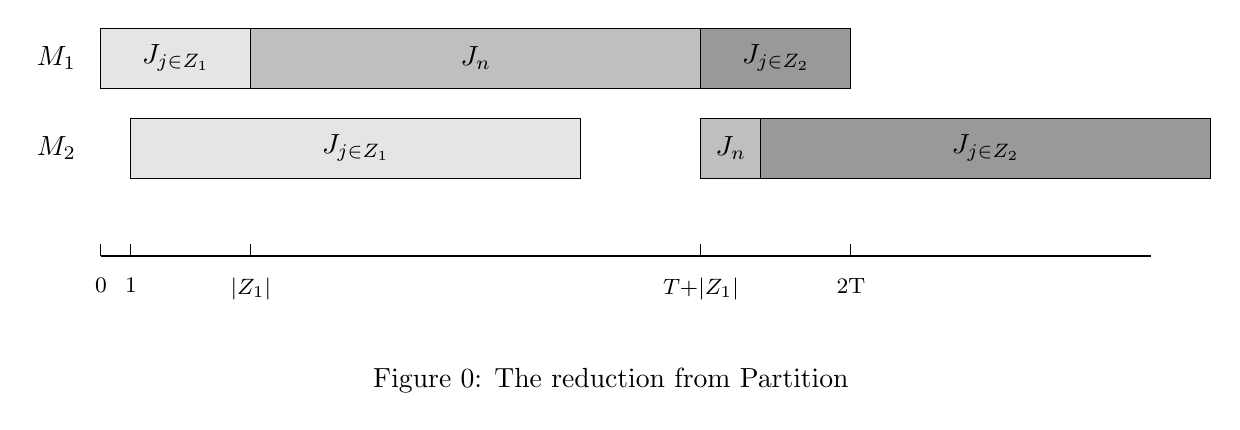
\begin{tikzpicture}[x=0.15in, y=0.3in]
	% machine index
	\node[anchor=east] at (-0.5,5.5) {$M_1$};
	\node[anchor=east] at (-0.5,4) {$M_2$};

	% job on M_1 (all 6 jobs in Johnson Sequence )
	\draw[fill=gray!20] (0,5)   rectangle (5,6)   node[midway] {$J_{j\in Z_1}$};
	\draw[fill=gray!50] (5,5)   rectangle (20,6)   node[midway] {$J_n$};
	\draw[fill=gray!80] (20,5)   rectangle (25,6)  node[midway] {$J_{j\in Z_2}$};

	% job on M_2 (all 6 jobs, start when M1 finishes and M2 is free)
	\draw[fill=gray!20] (1,3.5)  rectangle (16,4.5)  node[midway] {$J_{j\in Z_1}$};
	\draw[fill=gray!50] (20,3.5)  rectangle (22,4.5) node[midway] {$J_n$};
	\draw[fill=gray!80] (22,3.5) rectangle (37,4.5)  node[midway] {$J_{j\in Z_2}$};

	% x-axis
	\draw[thick] (0,2.2) -- (35,2.2);
	\foreach \x/\label in {0/0 ,1/1 ,5/$|Z_1|$ ,20/$T{+}|Z_1|$ ,25/2T ,}
    {
		\draw (\x,2.2) -- (\x,2.4);
		\node[below, font=\footnotesize] at (\x,2.0) {\label};
	}

	% caption
	\node[below] at (17,0.5) {Figure~\thefigure: The reduction from Partition};
\end{tikzpicture}
\label{fig:nphard-partition}
\end{figure}

Job $J_n$ splits the remaining jobs into two subsets, and \Cref{fig:nphard-partition} shows the
layout the split leaves on the two machines. The $M_2$ workloads of the subsets are unknown, but
they sum to $2rT$, so they can be written as $r(T+\xi)$ and $r(T-\xi)$ for some $-T\le\xi\le T$. The completion times of $J_n$ are then
\begin{equation}\label{eq:completetime1}
    C_n^1 = |Z_1| + rT + 1,
\end{equation}
\begin{equation}\label{eq:completetime2}
    C_n^2 = 1 + r(T+\xi) + 1,
\end{equation}
and $C_n = \max\{C_n^1, C_n^2\}$.

If $\xi=0$, the two subsets carry the same $M_2$ load, and the Partition instance has a solution.
In this case $C_n$ is given by \cref{eq:completetime1}, and
\begin{align*}
C_n &= |Z_1| + rT + 1 \le rT + r = r(T+1), \\
w_nC_n &= (2T+1)\,r(T+1) = Y, \\
W C_{\max} &= r(T+1)(C_n + rT) = Y,
\end{align*}
so $w_jC_j\le W C_{\max}=Y$.

Conversely, suppose that some schedule satisfies $W C_{\max}\le Y$. When $\xi>0$, $C_n$ is given by
\cref{eq:completetime2}, and
\begin{align*}
C_n &= 1 + r(T+\xi) + 1 \ge 1 + r(T+1) + 1, \\
w_nC_n &\ge (2T+1)\bigl(1 + r(T+1) + 1\bigr) = Y.
\end{align*}
When $\xi<0$, $C_n$ is given by \cref{eq:completetime1}, and
\begin{align*}
C_{\max} &= C_n + \sum_{j\in Z_2}b_j \\
         &= 1 + rT + |Z_1| + r(T-\xi) \\
         &\ge rT + r + rT \\
         &= r(2T+1) = Y, \\
WC_{\max} &\ge r(T+1)\bigl(r(2T+1)\bigr) = Y,
\end{align*}
so $W C_{\max}>Y$, a contradiction.

The Partition instance therefore admits a solution if and only if the constructed
$F2 \parallel W C_{\max}$ instance admits a schedule with $W C_{\max}\le Y$.
\end{proof}

\begin{theorem}\label{thm:snphard}
    $F2 \parallel W C_{\max}$ is strongly NP-hard.
\end{theorem}
\begin{proof}
We reduce from the strongly NP-complete 3-Partition problem: given $3m$ positive integers $x_1,\dots,x_{3m}$ and an integer $B$ 
satisfying $B/4 < x_i < B/2$ and $\sum_{i=1}^{3m}x_i=mB$, can the integers be partitioned into $m$ triples, each of sum $B$?

Let $R=3m+5$, $D=RB+4$, and $T=mD$. We construct an instance with $3m$ element jobs $J_1,\dots,J_{3m}$ 
and $m$ separator jobs $S_1,\dots,S_m$:
\begin{itemize}
  \item for every element job $J_j$, set $a_j=1$, $b_j=Rx_j+1$;
  \item for every separator job $S_k$, set $a_{S_k}=RB+1$, $b_{S_k}=1$.
\end{itemize}
All processing times are positive integers. For $k=1,\dots,m$, define $d_k=kD+1$ and let $Q=(T+2)^3$. Set
\[
 w_{S_k}=\left\lfloor\frac{Q}{d_k}\right\rfloor,
 \qquad
 w_j=\left\lfloor\frac{Q}{T}\right\rfloor\quad(j=1,\dots,3m),
\]
and use the decision threshold $Y=Q$. Since $d_k\le T+1$ and $Q\ge d_k(d_k+1)$, we have $\lfloor Q/d_k\rfloor>d_k$. 
Thus, for every $d\in\{d_1,\dots,d_m,T\}$ and every integer completion time $C$,
\begin{equation}\label{eq:deadline-encoding}
 \left\lfloor\frac{Q}{d}\right\rfloor C\le Q
 \quad\Longrightarrow\quad C\le d.
\end{equation}
Indeed, if $C\ge d+1$, write $Q=qd+r$ with $q=\lfloor Q/d\rfloor$ and $0\le r<d$. Then $q(d+1)=Q-r+q>Q$ because $q>d>r$.
Suppose first that the 3-Partition instance is a yes-instance. Let $G_1,\dots,G_m$ be triples with
$\sum_{J_j\in G_k}x_j=B$ for every $k$; each triple contains exactly three elements, since two of
its members sum to less than $B$ and four to more. Schedule
\[
G_1,S_1,G_2,S_2,\dots,G_m,S_m.
\]
The three element jobs in $G_k$ use $3$ units on $M_1$, and $S_k$ uses $RB+1$ units, so $S_k$ completes on $M_1$
at time $kD$. On $M_2$ the group $G_k$ occupies the machine from time $(k-1)D+1$, which is the
completion of $S_{k-1}$ for $k\ge2$ and that of the first element of the group on $M_1$ for $k=1$,
and it uses $RB+3$ units there; the last element of $G_k$ therefore completes at time $kD$. Thus
\[
 C_{S_k}=kD+1=d_k.
\]
Every element job completes on $M_2$ no later than $T=mD$. By the definition of the weights, all weighted completion times 
are at most $Q$, so $W C_{\max}\le Y$.

Conversely, suppose that a schedule $\pi$ satisfies $W C_{\max}\le Y$. Since the objective is regular,
the standard permutation-schedule property for two-machine flow shops \citep{baker1974introduction}
lets us restrict attention to permutation schedules. The separator jobs have identical processing
times, so if their positions are fixed, exchanging the labels of two separators that occur in the
wrong order cannot increase the maximum weighted completion time: $d_k$ rises with $k$, so
$w_{S_1}\ge w_{S_2}\ge\cdots\ge w_{S_m}$, and the exchange only moves a larger weight to an earlier
completion. We may consequently assume that the separators occur in the order $S_1,S_2,\dots,S_m$.
By \cref{eq:deadline-encoding},
\[
 C_{S_k}\le kD+1\quad(k=1,\dots,m),
 \qquad C_j\le T\quad(j=1,\dots,3m).
\]
No element job can occur after $S_m$. Indeed, if at least one element job did so, consider the last such element job. 
By the permutation-schedule property invoked above, the processing sequences on $M_1$ and $M_2$
coincide, so this job is also the last job on $M_1$. All $m$ separators and all $3m$ element jobs
therefore complete on $M_1$ no later than it, so its $M_1$ completion time is at least the total
$M_1$ processing time
\[
 m(RB+1)+3m=m(RB+4)=T.
\]
Its $M_2$ completion time would then be strictly greater than $T$, contradicting $C_j\le T$. The element
jobs are therefore partitioned into the $m$ groups $G_k$ lying between $S_{k-1}$ and $S_k$, where $S_0$
denotes the start of the schedule.
Put
\[
 B_k=\sum_{J_j\in G_k}x_j,
 \qquad E_k=\sum_{h=1}^{k}|G_h|,
 \qquad E_0=0.
\]
For $k=2,\dots,m$, the $M_2$ path gives
\begin{equation}\label{eq:path-m2}
 C_{S_k}\ge C_{S_{k-1}}+RB_k+|G_k|+1,
\end{equation}
while the $M_1$ path to $S_{k-1}$ gives
\begin{equation}\label{eq:path-m1}
 C_{S_{k-1}}\ge (k-1)(RB+1)+E_{k-1}+1.
\end{equation}
Combining \cref{eq:path-m2} and \cref{eq:path-m1} with $C_{S_k}\le kD+1$ yields
\begin{equation}\label{eq:group-bound}
 R(B_k-B)+E_k\le 3k,\qquad k=2,\dots,m.
\end{equation}
For $k=1$, the $M_2$ path and $C_{S_1}\le D+1$ similarly give
\begin{equation}\label{eq:group-bound-k1}
 R(B_1-B)+E_1\le4.
\end{equation}
Because $R=3m+5$, \cref{eq:group-bound} and \cref{eq:group-bound-k1} imply $B_k\le B$ for every
$k$. Otherwise $B_k\ge B+1$, and the respective left-hand side exceeds $3k$, or exceeds $4$ when
$k=1$. Since every element job belongs to one of the groups, $\sum_{k=1}^{m}B_k=mB$, and hence
$B_k=B$ for every $k$.
Finally, $B/4<x_j<B/2$ implies that a group with sum $B$ contains exactly three elements: at most two elements have sum strictly 
less than $B$, while at least four elements have sum strictly greater than $B$. Thus $G_1,\dots,G_m$ is a valid 3-partition.

The construction uses $4m$ jobs, and all processing times, weights and the threshold are bounded by a
polynomial in $m$ and $B$. Since 3-Partition remains NP-complete when $B$ is polynomially bounded in
$m$, this is a strong polynomial reduction, and $F2 \parallel W C_{\max}$ is strongly NP-hard.
\end{proof}
\begin{figure}[H]
\centering
\refstepcounter{figure}
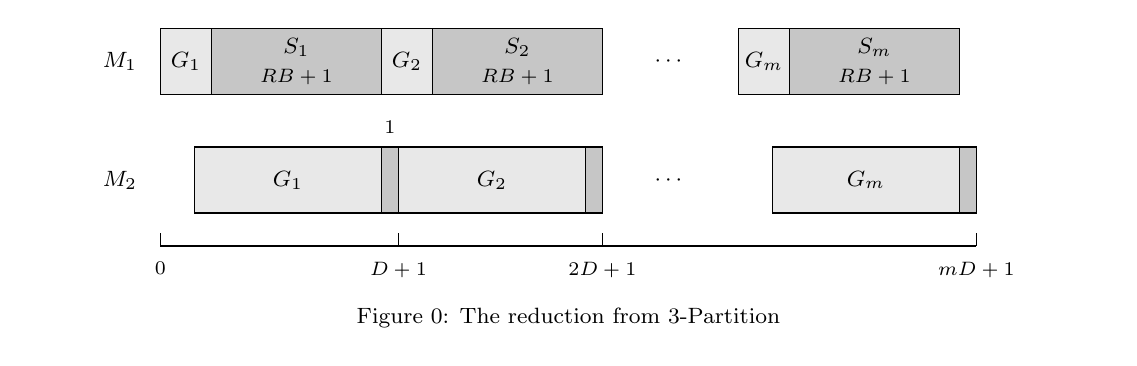
\begin{tikzpicture}[x=0.17in, y=0.33in, font=\footnotesize]
	\tikzset{
		elem/.style = {draw, fill=gray!18},
		sep/.style  = {draw, fill=gray!45},
	}
	% ---- M1: a group of three elements, then a separator -----------------
	\node[anchor=east] at (-0.4,5.7) {$M_1$};
	\draw[elem] (0,5.2)    rectangle (1.5,6.2) node[midway] {$G_1$};
	\draw[sep]  (1.5,5.2)  rectangle (6.5,6.2) node[midway, align=center] {$S_1$\\[-1pt]{\scriptsize $RB+1$}};
	\draw[elem] (6.5,5.2)  rectangle (8,6.2)   node[midway] {$G_2$};
	\draw[sep]  (8,5.2)    rectangle (13,6.2)  node[midway, align=center] {$S_2$\\[-1pt]{\scriptsize $RB+1$}};
	\node at (15,5.7) {$\cdots$};
	\draw[elem] (17,5.2)   rectangle (18.5,6.2) node[midway] {$G_m$};
	\draw[sep]  (18.5,5.2) rectangle (23.5,6.2) node[midway, align=center] {$S_m$\\[-1pt]{\scriptsize $RB+1$}};

	% ---- M2: the same groups, each closed by a separator of one unit -----
	\node[anchor=east] at (-0.4,3.9) {$M_2$};
	\draw[elem] (1,3.4)    rectangle (6.5,4.4) node[midway] {$G_1$};
	\draw[sep]  (6.5,3.4)  rectangle (7,4.4);
	\draw[elem] (7,3.4)    rectangle (12.5,4.4) node[midway] {$G_2$};
	\draw[sep]  (12.5,3.4) rectangle (13,4.4);
	\node at (15,3.9) {$\cdots$};
	\draw[elem] (18,3.4)   rectangle (23.5,4.4) node[midway] {$G_m$};
	\draw[sep]  (23.5,3.4) rectangle (24,4.4);
	\node[above, font=\scriptsize] at (6.75,4.45) {$1$};

	% ---- the separator completions that pin the groups -------------------
	\draw[thick] (0,2.9) -- (24,2.9);
	\foreach \x/\lab in {0/{$0$}, 7/{$D+1$}, 13/{$2D+1$}, 24/{$mD+1$}} {
		\draw (\x,2.9) -- (\x,3.1);
		\node[below, font=\scriptsize] at (\x,2.8) {\lab};
	}

	% ---- caption ---------------------------------------------------------
	\node[below, text width=13.5cm, align=flush center] at (12,2.1)
		{Figure~\thefigure: The reduction from 3-Partition};
\end{tikzpicture}
\label{fig:snphard-3partition}
\end{figure}

\section{Exact and approximation algorithms}
\label{sec:dp_algorithm}
This section develops the exact dynamic program and the two approximation algorithms that
rest on it. Throughout, $K$ denotes the number of distinct weights and
$V=\sum_{j=1}^{n}(a_j+b_j)$ the total processing time.

Since the objective is a maximum over weighted completion times, jobs of equal weight are
interchangeable. An optimal schedule can therefore be assumed to have a block structure:
one block per distinct weight, Johnson's order within each block, and blocks in
non-increasing weight order. A schedule is fixed once each weight class has been assigned to
a block, and the running time of every algorithm below is governed by the number $K$ of those
classes.

Three algorithms are built on this structure. The first is exact and prunes dominated states:
a state records each block's processing time on both machines, the completion time of its last
job on $M_2$, and that job's weight, and the dynamic program runs in
$O(n \cdot K \cdot |\mathscr{H}|_{\max})$ time with
$|\mathscr{H}|_{\max} \le 2^{K}V^{3K-3}$. The second sorts the jobs by non-increasing weight in
$O(n\log n)$ time and returns a schedule within a factor $2$ of the optimum. The third rounds
the time coordinates and the weights to geometrically spaced grids, which turns the dynamic
program into a $(1+\epsilon)$-approximation scheme for a fixed number of distinct weights.

\subsection{Block structure of an optimal schedule}
Within the permutation schedules of \Cref{sec:preliminaries}, Johnson's rule
\citep{johnson1954optimal} minimizes the makespan: the jobs with $a_j \le b_j$ are scheduled
first in non-decreasing order of $a_j$, and the remaining jobs follow in non-increasing order of
$b_j$.

Fix a permutation schedule $\pi$. Let $W_1 > W_2 > \cdots > W_K$ be the $K$ distinct weights
occurring among the jobs, and let
\[
\mathcal{G}_k = \{J_j \in \mathcal{J} \mid w_j = W_k\}, \qquad k = 1,\dots,K,
\]
denote the corresponding weight classes. Set $\ell_0 = 0$. For $k = 1,\dots,K$ in sequence, let
$\ell_k$ be the position of the last job of weight $W_k$ among the jobs not yet assigned to a block,
that is, among $\pi(\ell_{k-1}+1),\dots,\pi(n)$; if no such job remains, set $\ell_k = \ell_{k-1}$.
The blocks are the consecutive segments
\[
\mathcal{B}_k = \{\pi(\ell_{k-1}+1), \dots, \pi(\ell_k)\}, \qquad k = 1,\dots,K,
\]
so that in particular $\mathcal{B}_1 = \{\pi(1),\dots,\pi(\ell_1)\}$. Equivalently, once the blocks
$\mathcal{B}_1,\dots,\mathcal{B}_k$ have been removed, the remaining jobs are
\[
\mathcal{J}\setminus\bigcup_{i=1}^{k}\mathcal{B}_i = \{\pi(\ell_k+1),\dots,\pi(n)\}, \qquad k=1,\dots,K .
\]
Hence $\ell_1\le\ell_2\le\cdots\le\ell_K$, and no block extends beyond its own last job.
For each block $\mathcal{B}_i$, let $A_i$ and $B_i$ denote the total processing time of its jobs on
$M_1$ and $M_2$, respectively, $C_i$ the completion time of its last job on $M_2$, and $L_i$ the
weight of its last job. If $\ell_k = \ell_{k-1}$, then $\mathcal{B}_k$ contains no job; such a block
is called empty and satisfies $A_k = B_k = C_k = L_k = 0$, and it may host any job of weight at most
$W_k$. By construction, a non-empty block $\mathcal{B}_k$ ends with a job of weight $W_k$, whereas an
empty block has $L_k = 0$. Since $W_1 > W_2 > \cdots > W_K$, the block-end weights are non-increasing
on the non-empty blocks.

We illustrate the block construction with a small example.
\begin{exam}\label{ex:blocking}
Consider a six-job instance with sequence $\pi = (J_1, \dots, J_6)$ and the following $(a_j,b_j,w_j)$ values:
\[
\begin{array}{c|cccccc}
      & J_1 & J_2 & J_3 & J_4 & J_5 & J_6 \\
\hline
a_j &  2  &  5  &  6  &  8  &  4  &  3  \\
b_j &  5  &  7  &  9  &  4  &  3  &  2  \\
w_j &  2  &  2  &  5  &  2  &  4  &  2
\end{array}
\]

The weight classes are $\mathcal{G}_1=\{J_3\}$, $\mathcal{G}_2=\{J_5\}$, and
$\mathcal{G}_3=\{J_1,J_2,J_4,J_6\}$, and the resulting blocks are $\mathcal{B}_1=\{J_1,J_2,J_3\}$,
$\mathcal{B}_2=\{J_4,J_5\}$, and $\mathcal{B}_3=\{J_6\}$.
\end{exam}

\begin{figure}[H]
\centering
\refstepcounter{figure}
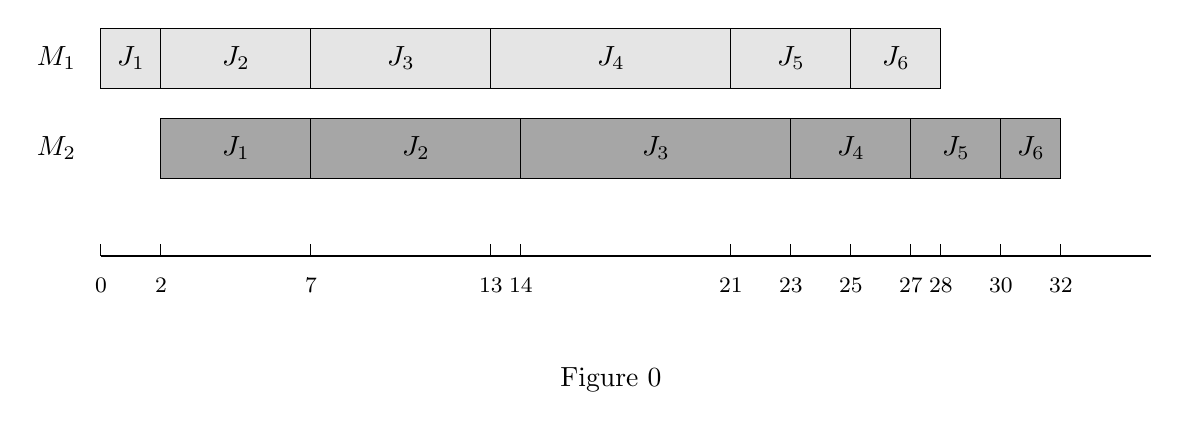
\begin{tikzpicture}[x=0.15in, y=0.3in]
	% machine index
	\node[anchor=east] at (-0.5,5.5) {$M_1$};
	\node[anchor=east] at (-0.5,4) {$M_2$};

	% job on M_1 (all 6 jobs in Johnson sequence)
	\draw[fill=gray!20] (0,5)   rectangle (2,6)   node[midway] {$J_1$};
	\draw[fill=gray!20] (2,5)   rectangle (7,6)   node[midway] {$J_2$};
	\draw[fill=gray!20] (7,5)   rectangle (13,6)  node[midway] {$J_3$};
	\draw[fill=gray!20] (13,5)  rectangle (21,6)  node[midway] {$J_4$};
	\draw[fill=gray!20] (21,5)  rectangle (25,6)  node[midway] {$J_5$};
	\draw[fill=gray!20] (25,5)  rectangle (28,6)  node[midway] {$J_6$};

	% job on M_2 (all 6 jobs, start when M1 finishes and M2 is free)
	\draw[fill=gray!70] (2,3.5)  rectangle (7,4.5)  node[midway] {$J_1$};
	\draw[fill=gray!70] (7,3.5)  rectangle (14,4.5) node[midway] {$J_2$};
	\draw[fill=gray!70] (14,3.5) rectangle (23,4.5) node[midway] {$J_3$};
	\draw[fill=gray!70] (23,3.5) rectangle (27,4.5) node[midway] {$J_4$};
	\draw[fill=gray!70] (27,3.5) rectangle (30,4.5) node[midway] {$J_5$};
	\draw[fill=gray!70] (30,3.5) rectangle (32,4.5) node[midway] {$J_6$};

	% x-axis
	\draw[thick] (0,2.2) -- (35,2.2);
	\foreach \x/\label in {0/0, 2/2, 7/7, 13/13, 14/14, 21/21, 23/23, 25/25, 27/27, 28/28, 30/30, 32/32} {
		\draw (\x,2.2) -- (\x,2.4);
		\node[below, font=\footnotesize] at (\x,2.0) {\label};
	}

	% caption
	\node[below] at (17,0.5) {Figure~\thefigure};
\end{tikzpicture}
\end{figure}

\begin{lemma}\label{lem:block-johnson}
For any schedule $\pi$, scheduling the jobs of each block by Johnson's rule~\citep{johnson1954optimal}
and concatenating the blocks in their original order gives a schedule $\pi'$ with
$W C_{\max}(\pi') \le W C_{\max}(\pi)$.
\end{lemma}
\begin{proof}
By construction, a non-empty block $\mathcal{B}_k$ ends with a job of weight $L_k$, and every job in
$\mathcal{B}_k$ has weight at most $L_k$: a weight occurring in $\mathcal{B}_k$ either equals $W_k$,
or it has already appeared in an earlier block, whose weights are larger. Let $C_{\pi(\ell_k)}$
denote the completion time of the last job of $\mathcal{B}_k$ in $\pi$, the job that sits at
position $\ell_k$. An empty block
satisfies $L_k C_{\pi(\ell_k)} = 0$ and therefore contributes nothing to the objective, so the
argument below applies to the non-empty blocks.

We first show that the maximum weighted completion time within a block is attained by the last job of
that block. For any $J_j \in \mathcal{B}_k$, the last job of the block completes no earlier than
$J_j$ in $\pi$, so $C_j \le C_{\pi(\ell_k)}$, while $w_j \le L_k$ by the block construction.
Hence
$w_j C_j \le L_k C_{\pi(\ell_k)}$, and taking the maximum over $j \in \mathcal{B}_k$ gives
\[
\max_{J_j \in \mathcal{B}_k} w_j C_j = L_k C_{\pi(\ell_k)}.
\]
The objective of \cref{eq:wcmax} therefore equals
\[
W C_{\max}(\pi) = \max_{k=1,\dots,K} L_k C_{\pi(\ell_k)},
\]
so it depends only on the last job of each block.

Let $\pi'$ be the schedule obtained by rescheduling the jobs within each block $\mathcal{B}_k$
according to Johnson's rule, keeping the blocks in their original order. We prove
$C_{\pi'(\ell_k)} \le C_{\pi(\ell_k)}$ for every $k$ by induction on $k$.

\textbf{Base case $k=1$.}
Block $\mathcal{B}_1$ starts at time zero on both machines regardless of its internal order, so
Johnson's rule gives $C_{\pi'(\ell_1)} \le C_{\pi(\ell_1)}$.

\textbf{Inductive step.}
Assume $C_{\pi'(\ell_{k-1})} \le C_{\pi(\ell_{k-1})}$. On $M_1$, the start time of $\mathcal{B}_k$
equals the
total $M_1$ work of $\mathcal{B}_1,\dots,\mathcal{B}_{k-1}$, which is invariant under internal
rescheduling, so $\mathcal{B}_k$ begins at the same instant on $M_1$ under both schedules. On $M_2$,
block $\mathcal{B}_k$ starts at $\max\{\sum_{i=1}^{k}A_{i},\,C_{\pi(\ell_{k-1})}\}$; the first term is
identical
under $\pi$ and $\pi'$, and the second is no larger under $\pi'$ by the induction hypothesis. Hence
$\mathcal{B}_k$ starts no later on $M_2$ under $\pi'$ than under $\pi$. Together with the same $M_1$
start and the internally optimal Johnson scheduling, this gives
$C_{\pi'(\ell_k)} \le C_{\pi(\ell_k)}$, which
completes the induction.

Finally,
\[
W C_{\max}(\pi') = \max_{k} L_k C_{\pi'(\ell_k)}
\le \max_{k} L_k C_{\pi(\ell_k)} = W C_{\max}(\pi),
\]
which establishes the lemma.
\end{proof}

\subsection{An exact dynamic program}
The exact dynamic program processes the jobs in the Johnson sequence and assigns each job to one
of the $K$ blocks $\mathcal{B}_1,\dots,\mathcal{B}_K$.

\Cref{lem:block-johnson} provides the structural basis for the dynamic program. Given any
assignment of jobs to the $K$ blocks, sequencing the jobs within each block $\mathcal{B}_i$
according to Johnson's rule and concatenating the blocks in the order of non-increasing block
weights yields a schedule whose $W C_{\max}$ value is no larger than that of any other schedule
respecting the same assignment.
For each $j = 1,\dots,n$, let $\mathscr{H}_j$ denote the set of states attainable after the first
$j$ jobs have been processed. A state records the following quantities for every block
$\mathcal{B}_i$:
\begin{itemize}
    \item $A_i$: the total processing time on machine $M_1$ of the jobs in block $\mathcal{B}_i$;
    \item $B_i$: the total processing time on machine $M_2$ of the jobs in block $\mathcal{B}_i$;
    \item $C_i$: the completion time of the last job of block $\mathcal{B}_i$ on machine $M_2$;
    \item $L_i$: the weight of the last job of block $\mathcal{B}_i$.
\end{itemize}
Since $W_1 > \cdots > W_K$, the blocks eligible for $J_j$ form a prefix. Writing
\[
    i^* = \max\{\, i : w_j \le W_i \,\},
\]
the eligible set is $\mathcal{E}(J_j) = \{\, 1,\dots,i^* \,\}$.
Each state is therefore the aggregate $K$-block tuple
\[
    (A_1,\dots,A_K; \; B_1,\dots,B_K; \; C_1,\dots,C_K; \; L_1,\dots,L_K),
\]
which is described by $4K$ parameters.

The initial state set contains a single state whose components are all zero:
$\mathscr{H}_{0} = \{ (0,\dots,0; \; 0,\dots,0; \; 0,\dots,0; \; 0,\dots,0) \}$.
In \Cref{alg:Block-concat}, $T_{A_i}$ denotes the total $M_1$ processing time of the first
$i$ blocks, and $T_{B_i}$ the completion time of block $\mathcal{B}_i$ on $M_2$.

\begin{lemma}\label{lem:merge-dominance}
Let $\mathscr{H} = (A_1,\dots,A_K; B_1,\dots,B_K; C_1,\dots,C_K; L_1,\dots,L_K)$ and
$\mathscr{H}' = (A'_1,\dots,A'_K; B'_1,\dots,B'_K; C'_1,\dots,C'_K; L'_1,\dots,L'_K)$ be two states
in $\mathscr{H}_j$. If $A_i = A'_i$, $B_i = B'_i$ and $L_i = L'_i$ for every $i$, and
$C_i \le C'_i$ for every $i$, then $\mathscr{H}'$ may be discarded without changing the optimal
value.
\end{lemma}
\begin{proof}
Consider any continuation that extends $\mathscr{H}'$ to a complete schedule $\Pi'$. Replacing the
prefix represented by $\mathscr{H}'$ with the prefix represented by $\mathscr{H}$ yields a schedule
$\Pi$ that assigns the remaining jobs identically. For every block $\mathcal{B}_k$ that follows the
updated one, the $M_2$ start time is $\max\{\sum_{i=1}^{k}A_{i},\, C_{k-1}\}$, and $C_{k-1}$ is no
larger under $\mathscr{H}$ than under $\mathscr{H}'$. By induction, the $M_2$ completion time of
every subsequent block is no larger under $\mathscr{H}$. Since $A_i$, $B_i$ and $L_i$ are identical
in the two states, the objective value $W C_{\max}$ of $\Pi$ does not exceed that of $\Pi'$.
\end{proof}

For $j = 1,\dots,n$, the algorithm extends $\mathscr{H}_{j-1}$ to $\mathscr{H}_j$ by placing $J_j$
at the end of each eligible block. That is, for every state in $\mathscr{H}_{j-1}$ and every
$i \in \mathcal{E}(J_j)$, only the $i$-th slice of the state is updated while all other blocks
remain unchanged:
\begin{equation}\label{eq:transition}
A'_i = A_i + a_j,\quad
B'_i = B_i + b_j,\quad
C'_i = \max\{C_i + b_j,\; A_i + a_j + b_j\}.
\end{equation}
The resulting candidate states are collected in temporary sets $\mathcal{Y}_1,\dots,\mathcal{Y}_K$.
By \Cref{lem:merge-dominance}, merging the candidates removes dominated and duplicate
states and yields $\mathscr{H}_{j}$.

\begin{algorithm}[H]
\small
\linespread{1.2}\selectfont
\SetAlgoLined
\DontPrintSemicolon
\caption{Block concatenation and evaluation}\label{alg:Block-concat}
\KwIn{State $\mathscr{H}=(A_1,\dots,A_K; B_1,\dots,B_K; C_1,\dots,C_K; L_1,\dots,L_K)$.}
\BlankLine
\textbf{Step 1.} [Initialization] Set $T_{A_0}\gets 0$, $T_{B_0}\gets 0$, $W C_{\max}\gets 0$. \;
\textbf{Step 2.} [Evaluation] \For{$i=1$ \KwTo $K$}{
    $T_{A_i}\gets T_{A_{i-1}}+A_i$ \;
    $T_{B_i}\gets \max\{\,T_{A_{i-1}}+C_i,\ T_{B_{i-1}}+B_i\,\}$ \;
    \If{$L_i>0$}{$W C_{\max}\gets \max\{\,W C_{\max},\ L_i\cdot T_{B_i}\,\}$ \;}
}
\KwOut{$W C_{\max}$.}
\end{algorithm}

\begin{algorithm}[H]
\small
\linespread{1.2}\selectfont
\SetAlgoLined
\DontPrintSemicolon
\caption{DP for $F2 \parallel W C_{\max}$}\label{alg:dp}
\KwIn{Jobs $\mathcal{J}$ with $(a_j,b_j,w_j)$; block count $K$; weights $W_1>\cdots>W_K$.}
\BlankLine
\textbf{Step 1.} [Initialization] Set $L_i\gets 0$ for $i=1,\dots,K$, set
	$\mathscr{H}_0\gets\{(0,\dots,0; \; 0,\dots,0; \; 0,\dots,0; \; 0,\dots,0)\}$ and $Z^{*}\gets+\infty$. \;
\textbf{Step 2.} [Generation] \For{$j=1$ \KwTo $n$}{
    \For{each $(A_1,\dots,A_K; B_1,\dots,B_K; C_1,\dots,C_K; L_1,\dots,L_K)\in\mathscr{H}_{j-1}$}{
        \For{each block $i\in\mathcal{E}(J_j)=\{1,\dots,i^{*}\}$}{
                $A_i'\gets A_i+a_j$, $B_i'\gets B_i+b_j$, $L_i'\gets w_j$ \;
                $C_i'\gets \max\{\,C_i+b_j,\ A_i+a_j+b_j\,\}$ \;
                Add the state 
                    $(A_1,\dots,A_i',\dots,A_K; B_1,\dots,B_i',\dots,B_K; C_1,\dots,C_i',\dots,C_K; L_1,\dots,L_i',\dots,L_K)$ 
                to $\mathscr{H}_j$ \;
			}
        }
    }
\textbf{[Elimination]} Elimination $\mathscr{H}_j$ for $j \in \{1,\dots,n\}$ by \Cref{lem:merge-dominance} \;
\textbf{Step 3.} [Calculate] \For{each state $S=(A_1,\dots,A_K; B_1,\dots,B_K; C_1,\dots,C_K; L_1,\dots,L_K)\in\mathscr{H}_n$}{
    \eIf{$L_i\in\{0,W_i\}$ for every $i=1,\dots,K$}{
        $W C_{\max}\gets$ \Cref{alg:Block-concat} applied to $S$ \;
        $Z^{*}\gets\min\{\,Z^{*},\ W C_{\max}\,\}$ \;
    }{
        Discard $S$. \;
    }
}
\textbf{Step 4.} [Result] Recover a schedule attaining $Z^{*}$ by standard backtracking. \;
\KwOut{An optimal schedule $\pi^{*}$.}
\end{algorithm}

To support Step~4, each state in $\mathscr{H}_j$ stores a pointer to the state in $\mathscr{H}_{j-1}$
from which it was derived, together with the block $i \in \mathcal{E}(J_j)$ into which $J_j$ was
placed. Starting from a state in $\mathscr{H}_n$ attaining $Z^{*}$, backtracking along these pointers
recovers the block $\mathcal{B}_i$ containing each job $J_j$. Sequencing the jobs of each block
according to Johnson's rule (\Cref{lem:block-johnson}) and concatenating the blocks then yields
an optimal schedule $\pi^{*}$ with $W C_{\max}(\pi^{*}) = Z^{*}$.

\begin{theorem}\label{thm:complexity}
\Cref{alg:dp} solves $F2 \parallel W C_{\max}$ optimally in
$O\bigl(n \cdot K \cdot |\mathscr{H}|_{\max}\bigr)$ time, where
$|\mathscr{H}|_{\max} \le 2^{K}V^{\,3K-3}$ and $V = \sum_{j=1}^{n}a_j + \sum_{j=1}^{n}b_j$.
For constant $K$, this is $O(nV^{\,3K-3})$.
\end{theorem}

\begin{proof}
Each state in $\mathscr{H}_j$ is the $4K$-tuple
\[
(A_1,\dots,A_K;\, B_1,\dots,B_K;\, C_1,\dots,C_K;\, L_1,\dots,L_K),
\]
so it suffices to bound the number of distinct values each component can attain.

The quantity $A_i$ is the total $M_1$ processing time of the jobs assigned to block
$\mathcal{B}_i$, hence $A_i \in [0,\,V]$. Since the $j$ jobs considered so far form a prefix of the
fixed Johnson sequence, $\sum_{i=1}^{K} A_i$ equals the sum of the $a_h$ over that prefix. At most
$K-1$ of the $A_i$ are therefore independent, contributing at most $V^{\,K-1}$ distinct
$A$-vectors. Symmetrically, $\sum_{i=1}^{K} B_i$ is the prefix sum of the $b_j$, so the $B_i$
components likewise contribute at most $V^{\,K-1}$ distinct combinations.

The quantity $C_i$ is the makespan of $\mathcal{B}_i$ when that block is scheduled in isolation by
Johnson's rule. Since $C_i \le A_i + B_i \le V$, the $C$-vector contributes at most $V^{K-1}$
distinct values. The weight $L_i$ equals $W_i$ when block $\mathcal{B}_i$ is non-empty and $0$ when
it is empty, so the $L$-vector takes at most $2^K$ distinct values. Multiplying these bounds gives
\[
|\mathscr{H}_{j}| \le 2^K \cdot V^{\,K-1} \cdot V^{\,2K-2} = 2^K \cdot V^{\,3K-3}.
\]

In iteration $j$, the algorithm takes each state in $\mathscr{H}_{j-1}$, tries every block
$i \in \{1,\dots,K\}$, computes the updated tuple in $O(1)$ time, and inserts it into
$\mathcal{Y}_i$. The merge step collects the $K$ sets $\mathcal{Y}_1,\dots,\mathcal{Y}_K$ and removes
duplicates in time proportional to the total number of generated tuples. Iteration $j$ therefore
costs $O(K \cdot |\mathscr{H}_{j-1}|)$, and summing over the $n$ iterations gives
$O(n \cdot K \cdot |\mathscr{H}|_{\max})$.

The final concatenation by \Cref{alg:Block-concat} evaluates each state in
$\mathscr{H}_{n}$ in $O(K)$ time, which is dominated by the DP phase. For fixed $K$, $2^K$ is
constant and the bound becomes $O(n \cdot V^{\,3K-3})$.
\end{proof}

\subsection{A 2-approximation}
\label{sub:approx2}

The exact dynamic program of \Cref{sec:dp_algorithm} runs in pseudo-polynomial
time, and the FPTAS of \Cref{sub:fptas} has running time exponential in the
number $K$ of distinct weights. When only a constant-factor guarantee is needed, the
following elementary rule suffices.

\begin{algorithm}[H]
\small
\linespread{1.2}\selectfont
\SetAlgoLined
\DontPrintSemicolon
\caption{2-Approximation for $F2 \parallel W C_{\max}$}\label{alg:approx2}
\KwIn{Jobs $\mathcal{J}$ with $(a_j,b_j,w_j)$.}
\BlankLine
\textbf{Step 1.} Sort the jobs by non-increasing weight $w_j$, breaking ties by non-increasing
$a_j+b_j$. \;
\textbf{Step 2.} Schedule the jobs in this sequence on both machines. \;
\KwOut{The resulting permutation schedule $\pi$.}
\end{algorithm}

\begin{theorem}\label{thm:approx2}
\Cref{alg:approx2} runs in $O(n\log n)$ time and returns a schedule with
$W C_{\max}\le 2\,W C_{\max}^{*}$.
\end{theorem}

\begin{proof}
Let $\pi$ be the schedule returned by \Cref{alg:approx2}. Its jobs appear in non-increasing
order of weight, so we name them $J_1,J_2,\dots,J_n$, with $w_1\ge w_2\ge\cdots\ge w_n$ and
$\pi=(J_1,J_2,\dots,J_n)$. Every job of the prefix $S=\{J_1,J_2,\dots,J_j\}$ then carries
a weight of at least $w_j$.

We first bound the completion times in $\pi$. By \cref{eq:completion}, the job $J_j$, which
sits at position $j$ of $\pi$, completes on $M_2$ at time $C_{\pi(j)}$, and every term of that
maximum is bounded by the
full sum:
\[
\sum_{h=1}^{i}a_h+\sum_{h=i}^{j}b_h
\le \sum_{h=1}^{j}a_h+\sum_{h=1}^{j}b_h
= \sum_{h\in S}\bigl(a_h+b_h\bigr),
\qquad 1\le i\le j.
\]
Hence
\begin{equation}\label{eq:approx2-completion}
C_{\pi(j)}\ \le\ \sum_{h\in S}\bigl(a_h+b_h\bigr).
\end{equation}
Since $W C_{\max}(\pi)=\max_{1\le j\le n}w_{\pi(j)}\,C_{\pi(j)}$ (\cref{eq:wcmax}), and
$w_{\pi(j)}=w_j$ for the job at position $j$, multiplying \cref{eq:approx2-completion}
by $w_j>0$ and taking the maximum over $j$ gives
\begin{equation}\label{eq:approx2-upper}
W C_{\max}(\pi)=\max_{1\le j\le n}w_{\pi(j)}\,C_{\pi(j)}
\le \max_{1\le j\le n}\,w_j\sum_{h\in S}\bigl(a_h+b_h\bigr).
\end{equation}

It remains to bound the right-hand side by $2W C_{\max}^{*}$. Fix a prefix
$S=\{J_1,J_2,\dots,J_j\}$ and let $\pi^{*}$ be an optimal schedule. Three quantities bound the
optimum from below,
\begin{equation}\label{eq:lb1}
LB_1=\max_{1\le j\le n}w_j\sum_{h\in S}a_h,
\end{equation}
\begin{equation}\label{eq:lb2}
LB_2=\max_{1\le j\le n}w_j\sum_{h\in S}b_h,
\end{equation}
\begin{equation}\label{eq:lb3}
LB_3=\max_{1\le j\le n}w_j\,(a_j+b_j),
\end{equation}
the $M_1$ threshold $LB_1$, the $M_2$ threshold $LB_2$ and the job threshold $LB_3$, and their
largest is the reference value of the instance,
\begin{equation}\label{eq:lb}
LB=\max\{LB_1,LB_2,LB_3\},
\end{equation}
so that $LB\le W C_{\max}^{*}$.

To see this, let $J_u$ be the job of $S$ that finishes last on $M_1$ in $\pi^{*}$, and $J_v$ the
job of $S$ that finishes last on $M_2$. All jobs of $S$ are processed on $M_1$ before $J_u$
completes $M_1$, so $C^{*}_u\ge\sum_{h\in S}a_h$. In the same way, all $M_2$ processing of the
jobs of $S$ precedes the completion of $J_v$ on $M_2$, so $C^{*}_v\ge\sum_{h\in S}b_h$. Since
both $J_u$ and $J_v$ lie in $S$, their weights satisfy $w_u,w_v\ge w_j$. The value
$W C_{\max}^{*}$ bounds the weighted completion time of every job of $\pi^{*}$, so
$W C_{\max}^{*}\ge w_u C^{*}_u\ge w_j\sum_{h\in S}a_h$ and
$W C_{\max}^{*}\ge w_v C^{*}_v\ge w_j\sum_{h\in S}b_h$. Every job $J_j$ of $S$ is processed on
$M_1$ before it is processed on $M_2$, and neither operation can be left out, so
$C^{*}_j\ge a_j+b_j$ and $W C_{\max}^{*}\ge w_jC^{*}_j\ge w_j(a_j+b_j)$. The prefix $S$ was
arbitrary, so these bounds hold for every prefix.

For the prefix $S$, the first two bounds give
$w_j\sum_{h\in S}(a_h+b_h)\le LB_1+LB_2\le 2\,LB\le 2\,W C_{\max}^{*}$, and the claim
follows from \cref{eq:approx2-upper}.
\end{proof}

\subsection{A fully polynomial-time approximation scheme}
\label{sub:fptas}

\subsubsection{Rounding the time coordinates}
\label{subsub:fptas-time}

The exact dynamic program of \Cref{alg:dp} becomes a fully polynomial-time approximation
scheme once the input data are rounded \citep{hall1994}. The technique rests on bounds for the
coordinates that are rounded: each time coordinate ranges over a bounded interval, and rounding
it to one of a fixed number of geometrically spaced values keeps the relative error within a
factor $\theta$. The total processing times $A_i,B_i$ of block $\mathcal{B}_i$ on $M_1$
and $M_2$, and its completion time $C_i$, are rounded. The weight $L_i$ of the
last job of block $\mathcal{B}_i$ is not rounded; following
\Cref{alg:dp}, the positional constraint $L_i\in\{0,W_i\}$ is required
for every block, and a state violating it is discarded.

Fix $0<\epsilon<1$ and let
\[
\theta=1+\frac{\epsilon}{2n},\qquad
V_A=\sum_{j=1}^{n}a_j,\qquad
V_B=\sum_{j=1}^{n}b_j,\qquad
V=V_A+V_B.
\]
For every block $\mathcal{B}_i$, the recurrence \cref{eq:transition}
preserves $A_i\le V_A$ and $B_i\le V_B$, since block $\mathcal{B}_i$ contains a
subset of the jobs; moreover $C_i\le A_i+B_i\le V$. We therefore round the $A$
dimension over $[0,V_A]$, the $B$ dimension over $[0,V_B]$, and the $C$
dimension over $[0,V]$. To this end, let
\[
\Delta(x)=k=\big\lfloor\log_\theta x\big\rfloor
\quad\text{for every }x\ge 1\text{ with }\theta^{k}\le x<\theta^{k+1},
\qquad\text{and}\qquad \Delta(0)=-1 .
\]
All processing times are integral, so every value taken by a coordinate
$A_i,B_i,C_i$ is a nonnegative integer. Hence any two values $y,y'\ge1$ with
$\Delta(y)=\Delta(y')$ satisfy $y\le\theta\,y'$; we call this the
\emph{interval-dominance} property, and it is the only fact about the rounding
used in the analysis below.

The \emph{label} of a
state $\mathscr{H}^{\epsilon}=(A_1,\dots,A_K; B_1,\dots,B_K; C_1,\dots,C_K; L_1,\dots,L_K)$
is the tuple formed by applying $\Delta$ to its time coordinates, together with its block-end weights,
\[
\ell(\mathscr{H}^{\epsilon})=
\bigl(\Delta(A_1),\dots,\Delta(A_K);\;
\Delta(B_1),\dots,\Delta(B_K);\;
\Delta(C_1),\dots,\Delta(C_K);\;
L_1,\dots,L_K\bigr).
\]
Thus two states share a label exactly when every coordinate $A_i$, $B_i$ and
$C_i$ falls into the same box and their block-end weights coincide. Each dimension
$x\in\{A,B,C\}$ contributes at
most $v^{x}+2$ distinct values of $\Delta$, where
$v^{x}=\lceil\log_\theta V_x\rceil$ and $V_C=V$, while the weight is not rounded and
each $L_i$ takes at most $n+1$ values.

The Elimination step keeps one representative per label. At iteration $j$, every state of
$\mathscr{H}^{\epsilon}_{j-1}$ spawns one candidate for each eligible block
$i\in\mathcal{E}(J_j)=\{1,\dots,i^{*}\}$, and each candidate is assigned its label. Two
candidates with the same label are indistinguishable after rounding and carry the same
block-end weights $L_1,\dots,L_K$, so the step keeps any one of them and discards the rest:
the kept state satisfies $x\le\theta\,\tilde x$ in every time coordinate $x\in\{A,B,C\}$ of every
block, relative to every candidate $\tilde{\mathscr{H}}^{\epsilon}$ it replaces, while its
block-end weights are unchanged. Every
label therefore carries exactly one state into $\mathscr{H}^{\epsilon}_{j}$, and the number of
states never exceeds the number of labels.

\begin{algorithm}[H]
\small
\linespread{1.2}\selectfont
\SetAlgoLined
\DontPrintSemicolon
\caption{State-class FPTAS for $F2 \parallel W C_{\max}$}\label{alg:fptas}
\KwIn{Jobs $\mathcal{J}$ with $(a_j,b_j,w_j)$; block count $K$; accuracy $\epsilon$.}
\BlankLine
\textbf{Step 1.} [Initialization] Set $\theta=1+\epsilon/(2n)$; set $Z^{*}\gets+\infty$; 
			 $\mathscr{H}^{\epsilon}_{0}\gets\{(0,\dots,0; \; 0,\dots,0; \; 0,\dots,0; \; 0,\dots,0)\}$. \;
\textbf{Step 2.} [Generation] \For{$j=1$ \KwTo $n$}{
    \For{each state $(A_1,\dots,A_K; B_1,\dots,B_K; C_1,\dots,C_K; L_1,\dots,L_K)\in\mathscr{H}^{\epsilon}_{j-1}$}{
        \For{each block $i\in\mathcal{E}(J_j)=\{1,\dots,i^{*}\}$}{
            $\tilde A_i=A_i+a_j$, $\tilde B_i=B_i+b_j$, $\tilde L_i=w_j$ \;
            $\tilde C_i=\max\{\,C_i+b_j,\ A_i+a_j+b_j\,\}$ \;
            \textbf[Label] Record the label
            $\ell(\tilde{\mathscr{H}}^{\epsilon}_{j})=\bigl(\Delta(\tilde A_1),\dots,\Delta(\tilde A_K);\;
            \Delta(\tilde B_1),\dots,\Delta(\tilde B_K);\;
            \Delta(\tilde C_1),\dots,\Delta(\tilde C_K);\;
            \tilde L_1,\dots,\tilde L_K\bigr)$. \;
        }
        \textbf [Elimination] Among the candidate states sharing the same label, keep one of them and
            delete the others;
            set $\mathscr{H}^{\epsilon}_{j}$ to the kept states. \;
    }
}
\textbf{Step 3.} [Calculate] Same as Step~3 of \Cref{alg:dp}, applied to $\mathscr{H}^{\epsilon}_{n}$. \;
\textbf{Step 4.} [Result] Same as Step~4 of \Cref{alg:dp}. \;
\KwOut{An approximate schedule $\pi$.}
\end{algorithm}

\begin{lemma}\label{lem:traj-approx}
Let $\mathscr{H}_{j}=(A_1,\dots,A_K; B_1,\dots,B_K; C_1,\dots,C_K; L_1,\dots,L_K)$, $j=1,\dots,n$, be the
states along an optimal trajectory of \Cref{alg:dp}, the states that backtracking from an optimal
final state recovers. For every $j$, \Cref{alg:fptas} keeps a state
$\hat{\mathscr{H}}^{\epsilon}_{j}=(\hat A_1,\dots,\hat A_K; \hat B_1,\dots,\hat B_K; \hat C_1,\dots,\hat C_K; L_1,\dots, L_K)$
that carries the same block-end weights $L_1,\dots,L_K$ and satisfies
\begin{equation}\label{eq:traj-bound}
\hat A_i\le A_i\,\theta^{j-1},~~
\hat B_i\le B_i\,\theta^{j-1},~~
\hat C_i\le C_i\,\theta^{j-1},~~(1\le i\le K).
\end{equation}
\end{lemma}

\begin{proof}
We argue by induction on $j$, from $1$ to $n$.

\textbf{Base case $j=1$.} Both algorithms generate their candidates for $J_1$ from the same zero
state. Two candidates that place $J_1$ in different blocks differ in at least one time coordinate,
so they carry different labels and no state is deleted. The sets $\mathscr{H}^{\epsilon}_{1}$ and
$\mathscr{H}_{1}$ therefore coincide, and \cref{eq:traj-bound} holds with equality at $j=1$.

\textbf{Inductive step $j\ge2$.} Assume that \cref{eq:traj-bound} holds at $j-1$, and let $i$ be the
block to which $\mathscr{H}_{j-1}$ appends $J_j$ in \Cref{alg:dp}. \Cref{alg:dp}
assigns a job only to a block $i$ with $w\le W_i$, so $w_j\le W_i$. This constraint depends only on
$J_j$ and the block index, hence appending $J_j$ to block $i$ is available from
$\hat{\mathscr{H}}^{\epsilon}_{j-1}$ as well. Write $A^{\prime}_i$, $B^{\prime}_i$ and $C^{\prime}_i$
for the coordinates of $\mathscr{H}_{j-1}$. Applying the exact recurrences to
$\hat{\mathscr{H}}^{\epsilon}_{j-1}$ and using $\theta^{j-2}\ge1$ gives a candidate
$\tilde{\mathscr{H}}^{\epsilon}_{j}$ with
\begin{align*}
\tilde A_{i} &= \hat A_{i}+a_j
   \le \big(A^{\prime}_{i}+a_j\big)\theta^{j-2}=A_{i}\theta^{j-2},\\
\tilde B_{i} &= \hat B_{i}+b_j
   \le \big(B^{\prime}_{i}+b_j\big)\theta^{j-2}=B_{i}\theta^{j-2},\\
\tilde C_{i} &= \max\big\{\hat C_{i}+b_j,\ \hat A_{i}+a_j+b_j\big\}\\
   &\le \max\big\{C^{\prime}_{i}+b_j,\ A^{\prime}_{i}+a_j+b_j\big\}\theta^{j-2}
   = C_{i}\theta^{j-2},
\end{align*}
where $A_i$, $B_i$ and $C_i$ are the coordinates of $\mathscr{H}_{j}$. For the remaining blocks
$m\ne i$ the same transition leaves the coordinates unchanged, so that
$\tilde x_m=\hat x_m\le x^{\prime}_m\theta^{j-2}=x_m\theta^{j-2}$ for $x\in\{A,B,C\}$. Hence
$\tilde x_m\le x_m\theta^{j-2}$ holds for every block $m=1,\dots,K$. The block-end weights
$L_1,\dots,L_K$ of the candidate are those of $\mathscr{H}_{j}$, because $L_i=w_j$ and the
remaining block-end weights are unchanged.

The candidate $\tilde{\mathscr{H}}^{\epsilon}_{j}$ carries the label
$\ell(\tilde{\mathscr{H}}^{\epsilon}_{j})$ assigned in \Cref{alg:fptas}, and the algorithm
keeps a state $\hat{\mathscr{H}}^{\epsilon}_{j}\in\mathscr{H}^{\epsilon}_{j}$ with that same label.
Since the label records the block-end weights, $\hat{\mathscr{H}}^{\epsilon}_{j}$ carries
$L_1,\dots,L_K$ as well. Interval dominance states that two values with the same index $\Delta$
differ by at most a factor $\theta$, so $y^{x}_{m}\le\theta\,\tilde x_{m}$ for every
$x\in\{A,B,C\}$ and every block $m=1,\dots,K$, where $y^{x}_{m}$ denotes the coordinates of
$\hat{\mathscr{H}}^{\epsilon}_{j}$. Together with $\tilde x_m\le x_m\theta^{j-2}$, this yields
\cref{eq:traj-bound} at $j$ and completes the induction.

Every state of $\mathscr{H}^{\epsilon}_n$ stores all $3K$ time coordinates, so the induction covers
the coordinates of the last block $\mathcal{B}_K$ as well. Storing these coordinates for every
block, exactly as in \Cref{alg:dp}, rather than deriving them from the others, preserves
the factor $\theta^{j-1}$ of \cref{eq:traj-bound}: a derived value would accumulate the rounding
errors of the remaining blocks.
\end{proof}

\begin{theorem}\label{thm:fptas}
For every $0<\epsilon<1$, \Cref{alg:fptas} returns a schedule with
\[
W C_{\max}\ \le\ (1+\epsilon)\,W C_{\max}^{*}.
\]
For fixed $K$, it runs in
$
O\!\left(n^{4K+1}\cdot K\cdot\frac{(\log V)^{3K}}{\epsilon^{3K}}\right)
$
time, which is polynomial in $n$, $\log V$ and $1/\epsilon$.
\end{theorem}

\begin{proof}
We first bound the value of the returned schedule, and then its running time.

Let $\mathscr{H}_{n}$ be the final state of the optimal trajectory of \Cref{alg:dp}, and let
$\hat{\mathscr{H}}^{\epsilon}_{n}\in\mathscr{H}^{\epsilon}_{n}$ be the state guaranteed by
\Cref{lem:traj-approx} at $j=n$. By the lemma, the time coordinates of
$\hat{\mathscr{H}}^{\epsilon}_{n}$ are within a factor $\theta^{n-1}$ of those of $\mathscr{H}_{n}$,
and its block-end weights are those of $\mathscr{H}_{n}$, because the weights are not rounded. The
final state $\mathscr{H}_{n}$ satisfies the positional constraint $L_i\in\{0,W_i\}$ of
\Cref{alg:dp}, so every block of $\hat{\mathscr{H}}^{\epsilon}_{n}$ has block-end weight at
most $W_i$.

Let $\hat\pi$ and $\pi^{*}$ be the schedules obtained by concatenating the blocks of
$\hat{\mathscr{H}}^{\epsilon}_{n}$ and $\mathscr{H}_{n}$, and let $\hat C_i$ and $C_i$ denote the
completion times of the last job of block $\mathcal{B}_i$ in the two schedules, which are the
corresponding coordinates of the two states. By the concatenation
recurrence of \Cref{alg:Block-concat}, $C_i$ is nondecreasing in every coordinate
of the state and positively homogeneous. Hence $\hat C_i\le\theta^{n-1}C_i$ for
every $i$. Since every block of $\hat{\mathscr{H}}^{\epsilon}_{n}$ has block-end weight at most
$W_i$, \Cref{lem:block-johnson} yields
\[
W C_{\max}(\hat\pi)
=\max_{1\le i\le K}W_i\,\hat C_i
\le \theta^{n-1}\max_{1\le i\le K}W_i\,C_i
=\theta^{n-1}\,W C_{\max}^{*}.
\]
The factor $\theta^{n-1}$ is at most $1+\epsilon$ for $0<\epsilon<1$. Because $1+x\le e^{x}$ for
every real $x$,
\[
\theta^{n-1}=\Bigl(1+\frac{\epsilon}{2n}\Bigr)^{n-1}
\le e^{\frac{(n-1)\epsilon}{2n}}
<e^{\epsilon/2},
\]
where the strict inequality uses $(n-1)/(2n)<1/2$. It is therefore enough to check that
$e^{\epsilon/2}\le1+\epsilon$ on $[0,1]$. The function $g(\epsilon)=1+\epsilon-e^{\epsilon/2}$
satisfies $g(0)=0$ and
\[
g'(\epsilon)=1-\tfrac12 e^{\epsilon/2}\ge 1-\tfrac12 e^{1/2}>0
\qquad(0\le\epsilon\le1),
\]
because $e^{\epsilon/2}\le e^{1/2}<2$ on that interval. Hence $g$ is increasing, so
$g(\epsilon)\ge0$ and $e^{\epsilon/2}\le1+\epsilon$. Consequently $\theta^{n-1}\le1+\epsilon$, and
the schedule returned by \Cref{alg:fptas}, being no worse than $\hat\pi$, has a value of
at most $(1+\epsilon)\,W C_{\max}^{*}$.

We now bound the running time. At each level $j$, \Cref{alg:fptas} keeps at most one state
per label, and the number of labels is $(v^{A}+2)^K(v^{B}+2)^K(v^{C}+2)^K(n+1)^K$. The rounded time
coordinates contribute $(v^{A}+2)^K(v^{B}+2)^K(v^{C}+2)^K$, which is at most $(v^{C}+2)^{3K}$ since
$v^{A},v^{B}\le v^{C}$, and each of the $K$ block-end weights takes at most $n+1$ values. Each
state generates at most $K$ candidates, one per eligible block, in $O(1)$ time each. The final
evaluation of the states of $\mathscr{H}^{\epsilon,n}$ costs $O(K)$ per state. The running time is
therefore $O\bigl(nK\,(v^{C}+2)^{3K}(n+1)^{K}\bigr)$. Since
$\ln(1+\epsilon/(2n))\ge\epsilon/(4n)$ for $0<\epsilon<1$, we have
\[
v^{C}=\Big\lceil\frac{\ln V}{\ln\theta}\Big\rceil
=O\!\left(\frac{n\log V}{\epsilon}\right).
\]
For constant $K$, the bound reduces to
$O(n^{4K+1}K(\log V)^{3K}/\epsilon^{3K})$, which is polynomial in $n$, $\log V$ and $1/\epsilon$.
\end{proof}

\subsubsection{Rounding the weights}
\label{subsub:fptas-weight}

The FPTAS above rounds the time coordinates $A_i,B_i,C_i$ and assumes that the number $K$ of
distinct weights is fixed. An analogous geometric rounding applies to the weights themselves when
their ratio is bounded. Let $W_{\min}=\min_{j}w_j$, $W_{\max}=\max_{j}w_j$, and suppose
$W_{\max}/W_{\min}\le c$ for a constant $c$. Partition the interval $[W_{\min},W_{\max}]$ into
\[
J_0=[W_{\min},W_{\min}\theta),\qquad
J_r=[W_{\min}\theta^{r},W_{\min}\theta^{r+1})\ \ (1\le r\le q-1),\qquad
J_q=[W_{\min}\theta^{q},W_{\max}],
\]
with $q=\big\lceil\log_\theta(W_{\max}/W_{\min})\big\rceil$, and round each weight $w_j$ upward to
the right endpoint of its interval,
\[
\hat w_j=W_{\min}\,\theta^{\,r_j+1},\qquad
r_j=\Big\lfloor\log_\theta\frac{w_j}{W_{\min}}\Big\rfloor,
\]
so that $w_j\le\hat w_j\le\theta\,w_j$. The rounded weights take only
$q+1=O\big(\log_\theta(W_{\max}/W_{\min})\big)$ distinct values, so jobs whose weights differ by a
factor at most $\theta$ merge into a single class.

\begin{lemma}\label{lem:weight-approx}
Let $\hat w_j$ be the rounded weights defined above, and let $\hat\pi$ be an optimal schedule of
the instance with weights $\hat w_j$, whose optimal value is $\hat W C_{\max}^{*}$. Then
\begin{equation}\label{eq:weight-bound}
W C_{\max}(\hat\pi)\le\theta\,W C_{\max}^{*}.
\end{equation}
\end{lemma}

\begin{proof}
By construction $w_j\le\hat w_j\le\theta w_j$ for every job $J_j$. By \cref{eq:wcmax} and the
monotonicity of the maximum,
every schedule $\pi$ satisfies
\[
W C_{\max}(\pi)=\max_{1\le j\le n}w_{\pi(j)} C_{\pi(j)}
\le\max_{1\le j\le n}\hat w_{\pi(j)} C_{\pi(j)}=\hat W C_{\max}(\pi)
\le\theta\,W C_{\max}(\pi).
\]
Let $\pi^{*}$ be an optimal schedule of the original instance. The rounded problem is solved
optimally by $\hat\pi$, and $\pi^{*}$ is feasible for it, so
\[
W C_{\max}(\hat\pi)\le\hat W C_{\max}(\hat\pi)=\hat W C_{\max}^{*}
\le\hat W C_{\max}(\pi^{*})\le\theta\,W C_{\max}(\pi^{*})=\theta\,W C_{\max}^{*},
\]
which is \cref{eq:weight-bound}.
\end{proof}

Hence the weight rounding incurs
a relative error of at most $\theta=1+\epsilon/(2n)\le 1+\epsilon$, exactly as in the
completion-time rounding.

\section{Heuristic algorithms}
\label{sec:heuristics}

The exact dynamic program of \Cref{sec:dp_algorithm} is pseudo-polynomial, and the
running time of the FPTAS of \Cref{sub:fptas} is exponential in the number $K$ of
distinct weights. Fast heuristics are therefore the practical route for large instances.
This section presents two of them for $F2 \parallel W C_{\max}$: an adaptation of the NEH
algorithm \citep{puka2024} and a genetic algorithm \citep{qiao2022adaptive}.

Throughout this section, the objective of a permutation
$\pi=(\pi(1),\dots,\pi(k))$ of $k$ jobs is evaluated by \cref{eq:completion} and
\cref{eq:wcmax}, so that
\[
W C_{\max}(\pi)=\max_{1\le t\le k} w_{\pi(t)}\, C_{\pi(t)},
\]
which is computed in $O(k)$ time.

\subsection{The NEH heuristic}
Constructive heuristics are attractive for $F2 \parallel W C_{\max}$ because they produce a
complete schedule in a single pass, without the tuning effort of population-based
metaheuristics. The NEH heuristic \citep{puka2024} is among the most effective
constructive rules for permutation flow shops, and its core idea is to build a schedule by
incrementally inserting jobs into a growing partial sequence, each time choosing the
position that best serves the objective.

In the maximum weighted completion-time objective, two properties are particularly
important. First, jobs with large total processing time $a_j+b_j$ tend to push the whole
makespan forward and therefore should appear early so as not to delay other jobs. Second,
given a fixed makespan, jobs with larger weight $w_j$ benefit more from occupying earlier
positions, because their weighted completion time decreases. These two properties suggest a
greedy priority in which large-$a_j+b_j$ jobs are placed first and large-$w_j$ jobs are used
as a tie-breaker.

We adapt the NEH framework as follows. The jobs are first sorted by non-increasing
$a_j+b_j$, breaking ties by non-increasing $w_j$, to obtain an initial sequence
$J_1,\dots,J_n$. The schedule starts with the single job $J_1$. For each $k=2,\dots,n$, the
next job $J_k$ is inserted into every one of the $k$ possible positions of the current
partial schedule. Each candidate sequence is evaluated by \cref{eq:completion}, and the
position that yields the smallest $W C_{\max}$ is retained. The pseudo-code is given in
\Cref{alg:neh}.

Because the partial schedule already contains $k-1$ jobs, the cost of evaluating all $k$
insertions at step $k$ is $O(k^2)$ using the recurrence \cref{eq:completion}; the total
running time is therefore $O(n^3)$ (\Cref{prop:neh-complexity}). The heuristic also
produces a feasible permutation schedule by construction and requires no hyperparameter
selection, so it serves as a fast standalone solver for large instances.

\begin{algorithm}[H]
\small
\linespread{1.2}\selectfont
\SetAlgoLined
\DontPrintSemicolon
\caption{NEH heuristic for $F2 \parallel W C_{\max}$}\label{alg:neh}
\KwIn{Jobs $\mathcal{J}$ with $(a_j,b_j,w_j)$.}
\BlankLine
\textbf{Step 1.} [Sequence] Sort the jobs by non-increasing $a_j+b_j$, breaking ties by $w_j$; 
let $J_{1},\dots,J_{n}$ be the resulting sequence. \;
\textbf{Step 2.} [Initialization] $\pi\gets(J_{1})$. \;
\textbf{Step 3.} [Insertion] \For{$k=2$ \KwTo $n$}{
    $\pi\gets$ the sequence obtained by inserting $J_{k}$ into $\pi$ at a position minimizing $W C_{\max}$. \;
}
\KwOut{Schedule $\pi$.}
\end{algorithm}

\begin{theorem}\label{prop:neh-complexity}
\Cref{alg:neh} runs in $O(n^3)$ time.
\end{theorem}
\begin{proof}
At step $k$, the job $J_{k}$ is inserted into each of the $k$ positions of a partial
schedule of $k-1$ jobs, and each candidate sequence is evaluated in $O(k)$ time by the
recurrence above. Hence step $k$ costs $O(k^2)$, and the total running time is
$O\bigl(\sum_{k=1}^{n}k^2\bigr)=O(n^3)$.
\end{proof}

\subsection{The genetic algorithm}
\label{sub:ga}

The objective $W C_{\max}$ is a bottleneck: a single \emph{critical} job attains the maximum
and fixes the value of a schedule. An ordering can therefore be improved in only two ways, by
lowering the completion time of that job or by shortening completion times across the board.
High-weight jobs should occupy early positions, so that their weighted completion stays small,
while the makespan should stay low so that no job is delayed unnecessarily, and a genetic
algorithm for $F2 \parallel W C_{\max}$ cannot treat the jobs symmetrically.

The genetic algorithm is a standard tool for flow-shop scheduling \citep{qiao2022adaptive}, and
it is used here within its classical framework, organised in four parts: the encoding and
decoding of a schedule, the generation of the initial population, the iteration of the
population, and the mutation of the offspring. Nothing in that framework is built around the
weight classes. The population starts from the order that is shortest on the two machines and
knows nothing of the weights, and it is the mutation that moves the blocks of one weight, one
block at a time, until the schedule carries the structure of \Cref{lem:block-johnson}.

\subsubsection{Encoding and decoding}
\textbf{Encoding.} A chromosome is a permutation $\pi=(\pi(1),\dots,\pi(n))$ of the $n$ jobs, in
which the gene at position $t$ is the job scheduled $t$-th. Its length is the number of jobs and
its alphabet the job set $\mathcal{J}$, and since both machines process the jobs in the order the
chromosome gives, every chromosome stands for a permutation schedule and every permutation
schedule for exactly one chromosome. No repair operator is therefore needed to restore feasibility
after crossover or mutation.

\textbf{Decoding.} Both machines process the jobs in the order $\pi(1),\dots,\pi(n)$. The
completion time $C_{\pi(t)}$ of the $t$-th job follows from the closed form
\cref{eq:completion}, which is evaluated in $O(n)$ time using the prefix sums
$A_t=\sum_{h=1}^{t}a_{\pi(h)}$ and $B_t=\sum_{h=1}^{t}b_{\pi(h)}$; the objective
value is that of \cref{eq:wcmax},
\[
W C_{\max}(\pi)=\max_{1\le t\le n}w_{\pi(t)}\,C_{\pi(t)}.
\]
The fitness of a schedule is the criterion itself, $W C_{\max}(\pi)$, and no normalised scale
is fixed for it. \Cref{fig:encoding} shows the encoding and
the decoding on the six-job instance of \Cref{ex:blocking}.

\begin{figure}[H]
\centering
\refstepcounter{figure}
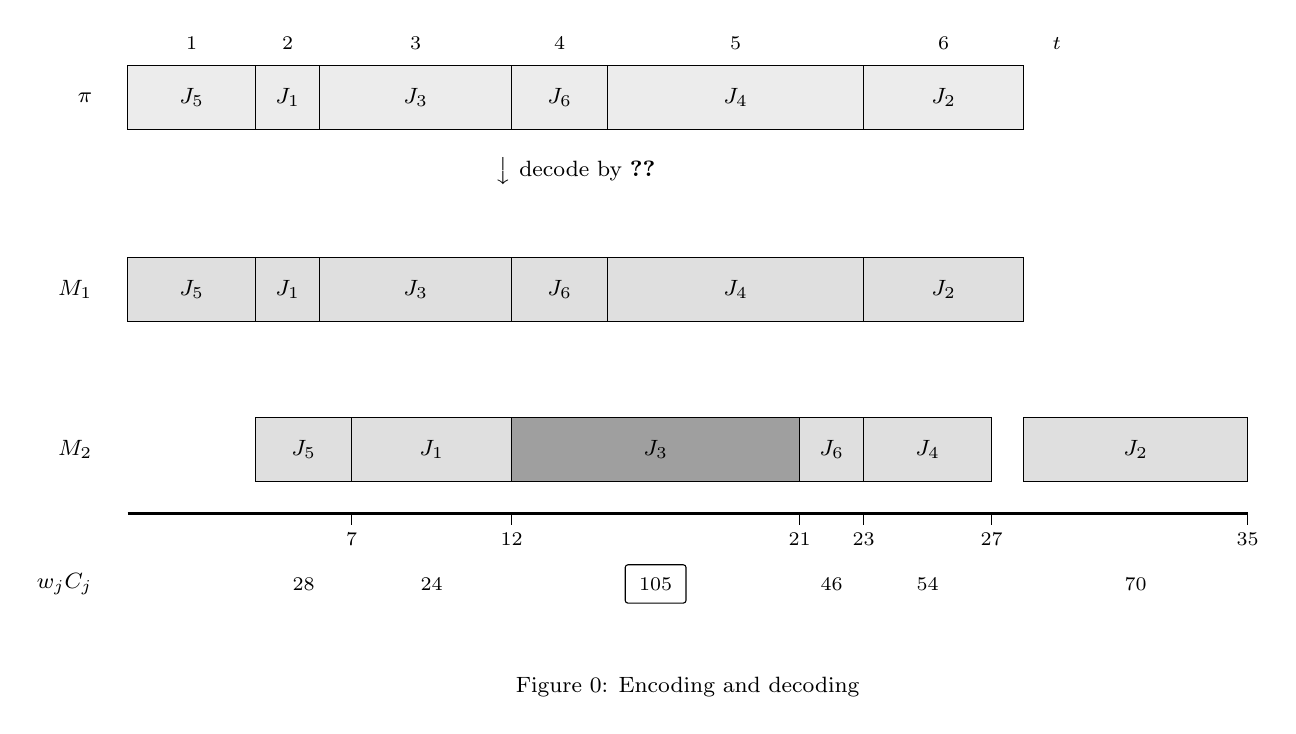
\begin{tikzpicture}[x=0.16in, y=0.32in, font=\footnotesize]
	% the chromosome: the gene at position t is the job scheduled t-th
	\node[anchor=east] at (-0.8,9.5) {$\pi$};
	\foreach \x/\y/\job/\t in {0/4/{$J_5$}/1, 4/6/{$J_1$}/2, 6/12/{$J_3$}/3,
	                           12/15/{$J_6$}/4, 15/23/{$J_4$}/5, 23/28/{$J_2$}/6} {
		\draw[fill=gray!15] (\x,9.0) rectangle (\y,10.0) node[midway] {\job};
		\node[font=\scriptsize] at ({(\x+\y)/2},10.35) {\t};
	}
	\node[anchor=west, font=\scriptsize] at (28.6,10.35) {$t$};

	% decoding
	\node at (14,8.35) {$\big\downarrow$ decode by \cref{eq:completion}};

	% M_1 processes the jobs in the order of the genes
	\node[anchor=east] at (-0.8,6.5) {$M_1$};
	\foreach \x/\y/\job in {0/4/{$J_5$}, 4/6/{$J_1$}, 6/12/{$J_3$},
	                        12/15/{$J_6$}, 15/23/{$J_4$}, 23/28/{$J_2$}} {
		\draw[fill=gray!25] (\x,6.0) rectangle (\y,7.0) node[midway] {\job};
	}

	% M_2 starts each job when M_1 has finished it and M_2 is free
	\node[anchor=east] at (-0.8,4.0) {$M_2$};
	\foreach \x/\y/\job/\c/\v/\f in {4/7/{$J_5$}/7/28/gray!25,
	                                 7/12/{$J_1$}/12/24/gray!25,
	                                 12/21/{$J_3$}/21/105/gray!75,
	                                 21/23/{$J_6$}/23/46/gray!25,
	                                 23/27/{$J_4$}/27/54/gray!25,
	                                 28/35/{$J_2$}/35/70/gray!25} {
		\draw[fill=\f] (\x,3.5) rectangle (\y,4.5) node[midway] {\job};
		\draw (\y,3.0) -- (\y,2.82);
		\node[font=\scriptsize] at (\y,2.6) {\c};
		\node[font=\scriptsize] at ({(\x+\y)/2},1.9) {\v};
	}
	\node[anchor=east] at (-0.8,1.9) {$w_jC_j$};
	\draw[rounded corners=1pt] (15.55,1.6) rectangle (17.45,2.2);
	\draw[thick] (0,3.0) -- (35,3.0);

	% caption
	\node[below, align=flush center] at (17.5,0.6) {Figure~\thefigure: Encoding and decoding};
\end{tikzpicture}
\label{fig:encoding}
\end{figure}

\subsubsection{Initial population}
Random starting populations waste most of the search effort.  The initial population $P_0$ of
size $N$ is therefore built from Johnson's rule \citep{johnson1954optimal}.  Its first
individual is the Johnson schedule $\pi^{\mathrm{J}}$ itself, which minimizes the makespan and
so shortens every completion time at once.  The remaining $N-1$ individuals are neighbours of
that schedule, each of them a copy of it with a few neighbouring jobs exchanged, the number of
exchanges being drawn uniformly between one and $\lfloor n/4\rfloor$.  A uniformly random
permutation carries nothing of the instance, while a neighbour of Johnson's order is already
short on the makespan.  The rule reads the two processing times alone and knows nothing of the
weights, so the population starts from the order that is shortest on the machines and the
criterion is brought in by the block move that follows, one weight at a time. The population
size grows with the instance and is capped, $N=\min(20,\max(6,\lceil n/2\rceil))$:
a small instance is given a small population, and a large one keeps the same twenty
individuals, which are enough for the block mutation and the local search to reach what
a population as large as the instance reaches. A generation is dominated by the mutation,
which evaluates $n$ positions of a block at $O(n)$ time each, and therefore costs
$O(\lambda n^{2})$, where $\lambda$ is the number of offspring the generation produces.

\subsubsection{Selection, crossover and survival}
A generation turns the population into its successor by three moves.  The parents are
selected, the parents are recombined into offspring, and the fittest of parents and
offspring survive.  The algorithm runs $G$ generations of them, and each of them produces
$\lambda$ offspring from its $N$ parents, so that the operators of one generation are run
several times over the same parents.  The population it starts from carries nothing of the
weights, so the generations are spent building the criterion into the schedule rather than
moving an order that already has it, and both $G$ and $\lambda$ rise with the instance: the
depth a run reaches grows with the number of generations, since the elite of one is a parent
of the next, and the number of classes an instance has to be sorted into does not.
A generation costs the evaluation of the $N+\lambda$ schedules it holds in $O(n)$ time each
and one pass of the operators over the offspring, whose most expensive move is the mutation of
a child in $O(n^{2})$, and the search therefore costs $O(G\lambda n^{2})$.  What is left of it
after the last generation is the local search that closes the algorithm.

\textbf{Selection.} Binary tournament selection forms the mating pool $M$. In each round, two
individuals are drawn uniformly at random from $P_{g-1}$. The better of
the two on the Pareto rank wins and is copied into the mating pool $M$, ties being broken by
the crowding distance. Both individuals are returned to the population, so that a parent may
be drawn more than once, and the round is repeated until $M_g$ contains $N$ individuals.
Tournament selection is preferred over roulette-wheel selection because it compares two
individuals directly rather than through a probability proportional to a fitness value. It
therefore
remains selective even as the population converges and the schedules of near-optimal
individuals become very close.

\textbf{Crossover.} The operator recombines two parent schedules into offspring. These inherit
both the relative order and the absolute positions of jobs, the two ingredients a permutation
schedule is built from. We use the partially mapped crossover (PMX), the standard operator for
permutation-encoded genetic algorithms. Two cut points $p_1<p_2$ are drawn uniformly at
random, and the middle segment $\pi_1[p_1..p_2]$ is copied verbatim into the child. The
remaining positions are filled from the second parent $\pi_2$. A gene $\pi_2[t]$ of such a
position $t\notin[p_1,p_2]$ clashes with the copy only when the copied segment already holds
it. The outer positions receive pairwise distinct genes of $\pi_2$, so no other clash is
possible, and a job cannot be written twice. Such a gene is replaced through the mapping that
the segment induces between the two parents, $j\gets\pi_2[\pi_1^{-1}(j)]$. The job $\pi_1$
holds at a segment position then gives way to the job $\pi_2$ holds at the same position. The
replacement is repeated while the gene it yields already occurs in the child. The mapping is
injective, so the chain it follows visits distinct jobs and stops after at most $p_2-p_1+1$
replacements. Every position then receives exactly one job, and the child is always a valid
permutation. PMX transfers contiguous blocks of jobs, which realize the front-heavy structure
identified in \Cref{sec:dp_algorithm}, while still recombining the two parents' orders on the
outer positions. Swapping the roles of
$\pi_1$ and $\pi_2$ yields the second child, so that one application replaces the two parents
by two offspring. \Cref{fig:pmx} shows both children of one application. Its two upper rows
are the parents and its two lower rows the offspring, the grey cells are the middle segment the
child copies ($\pi'$ takes the segment of $\pi_1$, $\pi''$ that of $\pi_2$), and the three
double arrows between the parents are the mapping the segment induces. The red cells, numbered
in the order in which they are visited, are those of the clash at position $1$ of $\pi'$: the
gene taken there, $\pi_2[1]=J_6$, is one the segment already holds, at position $3$, and the
chain $J_6\to J_1\to J_5$ stops at the free job $J_5$, which is the value the position
finally receives.

\begin{figure}[H]
\centering
\refstepcounter{figure}
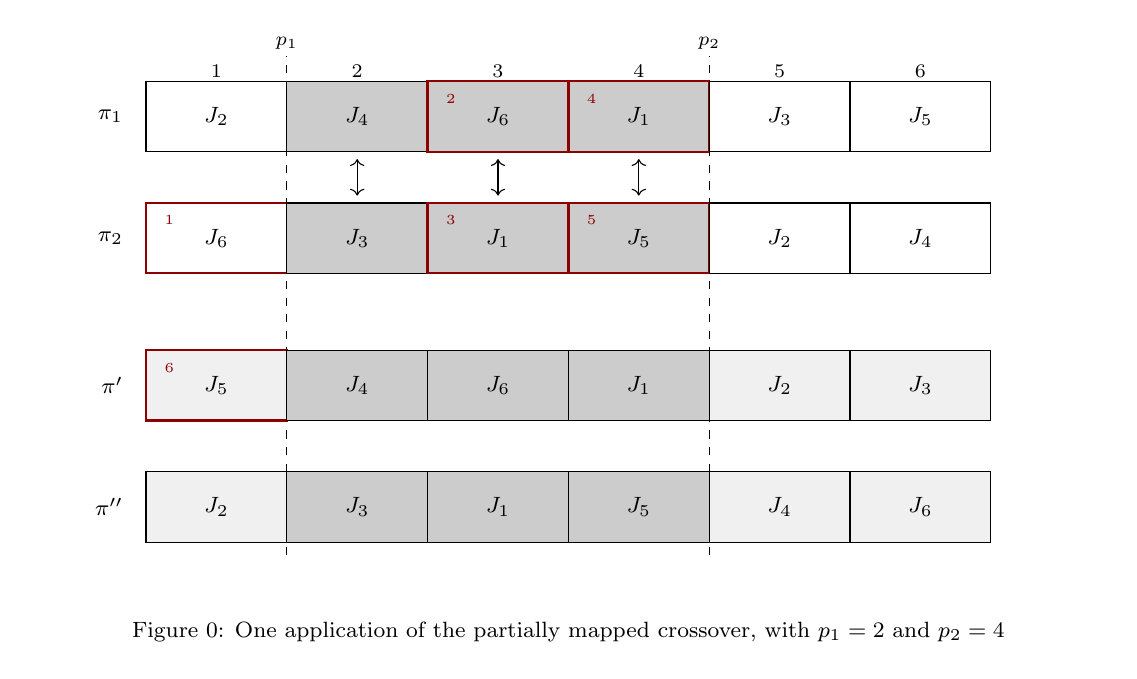
\begin{tikzpicture}[x=0.44in, y=0.32in, font=\footnotesize]
	% Two cues, kept apart on purpose: the grey fill marks the segment a child
	% inherits from one parent, and the red frame with the red path below marks
	% the cells that the clash at position 1 of the first child passes through.
	\tikzset{
		plaincell/.style = {draw},
		segcell/.style   = {draw, fill=gray!40},
		fillcell/.style  = {draw, fill=gray!12},
		clashcell/.style = {draw=red!55!black, thick},
		plainclash/.style = {plaincell, clashcell},
		segclash/.style   = {segcell, clashcell},
		fillclash/.style  = {fillcell, clashcell},
	}
	% ---- the two parents -----------------------------------------------------
	\node[anchor=east] at (-0.15,7.15) {$\pi_1$};
	\foreach \t/\job/\st in {1/{$J_2$}/plaincell, 2/{$J_4$}/segcell,
	                         3/{$J_6$}/segclash, 4/{$J_1$}/segclash,
	                         5/{$J_3$}/plaincell, 6/{$J_5$}/plaincell}
		\draw[\st] ({(\t-1)*1.6},6.6) rectangle ({\t*1.6},7.7) node[midway] {\job};
	\foreach \t in {1,...,6} \node[font=\scriptsize] at ({(\t-0.5)*1.6},7.85) {\t};

	\node[anchor=east] at (-0.15,5.25) {$\pi_2$};
	\foreach \t/\job/\st in {1/{$J_6$}/plainclash, 2/{$J_3$}/segcell,
	                         3/{$J_1$}/segclash, 4/{$J_5$}/segclash,
	                         5/{$J_2$}/plaincell, 6/{$J_4$}/plaincell}
		\draw[\st] ({(\t-1)*1.6},4.7) rectangle ({\t*1.6},5.8) node[midway] {\job};

	% the cut points of the segment, and the mapping it induces between them
	\foreach \x/\lab in {1.6/{$p_1$}, 6.4/{$p_2$}} {
		\draw[dashed] (\x,0.3) -- (\x,8.1);
		\node[font=\scriptsize] at (\x,8.3) {\lab};
	}
	\foreach \t in {2,3,4}
		\draw[<->, shorten >= 1.5pt, shorten <= 1.5pt]
			({(\t-0.5)*1.6},6.55) -- ({(\t-0.5)*1.6},5.85);

	% ---- the two offspring ---------------------------------------------------

	\node[anchor=east] at (-0.15,2.95) {$\pi'$};
	\foreach \t/\job/\st in {1/{$J_5$}/fillclash, 2/{$J_4$}/segcell,
	                         3/{$J_6$}/segcell, 4/{$J_1$}/segcell,
	                         5/{$J_2$}/fillcell, 6/{$J_3$}/fillcell}
		\draw[\st] ({(\t-1)*1.6},2.4) rectangle ({\t*1.6},3.5) node[midway] {\job};

	\node[anchor=east] at (-0.15,1.05) {$\pi''$};
	\foreach \t/\job/\st in {1/{$J_2$}/fillcell, 2/{$J_3$}/segcell,
	                         3/{$J_1$}/segcell, 4/{$J_5$}/segcell,
	                         5/{$J_4$}/fillcell, 6/{$J_6$}/fillcell}
		\draw[\st] ({(\t-1)*1.6},0.5) rectangle ({\t*1.6},1.6) node[midway] {\job};

	% the order in which the clash at position 1 of the first child visits the
	% red cells: 1 the gene taken from pi_2, 2 and 4 the cells of the segment that
	% already hold it, 3 and 5 the cells the mapping sends it to, 6 where it lands
	\foreach \x/\y/\k in {0/5.8/1, 3.2/7.7/2, 3.2/5.8/3, 4.8/7.7/4, 4.8/5.8/5,
	                      0/3.5/6}
		\node[anchor=north west, font=\tiny, text=red!55!black]
			at ({\x+0.1},{\y-0.05}) {\k};

	% caption
	\node[below, text width=13.5cm, align=flush center] at (4.8,-0.6) {Figure~\thefigure: One
		application of the partially mapped crossover, with $p_1=2$ and $p_2=4$};
\end{tikzpicture}
\label{fig:pmx}
\end{figure}

\begin{algorithm}[H]
\small
\linespread{1.2}\selectfont
\SetAlgoLined
\DontPrintSemicolon
\caption{Partially Mapped Crossover (PMX) for $F2 \parallel W C_{\max}$}\label{alg:pmx}
\KwIn{Parents $\pi_1,\pi_2$; cut points $p_1<p_2$.}
\BlankLine
\textbf{Step 1.} [Copy segment] Set $\pi'[t]\gets\pi_1[t]$ for $t=p_1,\dots,p_2$. \;
\textbf{Step 2.} [Fill outer positions] \For{$t=1$ \KwTo $n$, $t\notin[p_1,p_2]$}{
    $j\gets\pi_2[t]$ \;
    \While{$j$ occurs in $\pi'$}{
        $j\gets\pi_2[\pi_1^{-1}(j)]$ \tcp*{follow the PMX mapping}
    }
    $\pi'[t]\gets j$ \;
}
\KwOut{Child $\pi'$.}
\end{algorithm}

\textbf{Survival.} The parents of $P_{g-1}$ and the offspring $O_g$ are pooled, so that a good
incumbent is never discarded. The $N$ survivors of $P_{g-1}\cup O_g$ are chosen by the
non-dominated sorting and the crowding distance of NSGA-II
\citep{deb2002fast}. Those rank the pooled individuals on three quantities, the
makespan $C_{\max}(\pi)$ of the schedule, the weight $w_{\pi(n)}$ of the job that
closes it, and the criterion $W C_{\max}(\pi)$ itself. Whole Pareto fronts are kept while they
fit into the budget of $N$ individuals.
The front that overflows it is cut by the crowding distance, its least crowded individuals
first. The first two carry the criterion: the weighted completion
of the closing job is exactly their product,
\[
w_{\pi(n)}\,C_{\max}(\pi)\le W C_{\max}(\pi),
\]
so ranking on them keeps both its ingredients in view, a schedule that ends early and one
whose last job is light, and keeps the weights in the account, which a search that pressed the
makespan alone would leave out. They are not the criterion, however, since a schedule can end
early and light and still be a poor one, and a search that ranked them alone would spend its
selection on the trade-off between them rather than on what the method is measured on. The
criterion is therefore ranked with them rather than tracked beside them. It is also tracked
on its own, over every child of every generation, and the best schedule seen on it is carried
into the next generation: where the ranking does not keep it, it takes the place of the
individual the ranking leaves last, so that an improvement is a parent of the generation that
follows and not merely a value that was recorded once.

\subsubsection{Mutation}
The crossover reads nothing of the weights, so the mutation is what keeps the search moving
across the weights: it moves whole weights rather than single jobs, and it is what carries the
population across the block orders the criterion rewards.

The move is the one the block structure of \Cref{lem:block-johnson} suggests.  An optimal
schedule holds one block per distinct weight, the blocks in non-increasing order of it, and
the arrangement the search has to reach is therefore an order of the blocks rather than of the
jobs.  A single job moved at a time cannot reach it quickly: placing one job leaves the other
jobs of its weight where they were, so the search would need as many accepted moves as there
are jobs.  The mutation therefore moves a block.  The jobs of one weight leave the schedule,
keeping the order they hold in it, and the run is put back at the position that minimizes
$W C_{\max}$ over the whole schedule, which is evaluated by \cref{eq:completion} at every one
of the positions the run can take.  The weight is the one of a job attaining
$W C_{\max}(\pi)$, since that is the job that closes the criterion, and with probability
$1/2$ a weight drawn at random is used instead, so that the order of the blocks is explored and
not only repaired.

The move is a variation and not an improvement.  Moving a block forward delays every job it
passes, so the criterion may rise while the block order moves towards the one
\Cref{lem:block-johnson} prescribes, and there are orders the criterion rewards that no
sequence of accepted moves reaches.  The move is therefore proposed whether or not it lowers
the criterion, and it is the survival of the generation, and the elite carried through it,
that decide what becomes of it.

\begin{algorithm}[H]
\small
\linespread{1.2}\selectfont
\SetAlgoLined
\DontPrintSemicolon
\caption{Block Mutation for $F2 \parallel W C_{\max}$}\label{alg:cm}
\KwIn{Schedule $\pi$; weights $w_j$.}
\BlankLine
\textbf{Step 1.} [Block] Evaluate $W C_{\max}(\pi)$ by \cref{eq:completion} and let $j^{*}$ be
a job attaining the maximum; with probability $1/2$ let $W\gets w_{j^{*}}$, otherwise let
$W$ be a weight drawn at random from the instance. \;
\textbf{Step 2.} [Move] Form the run of the jobs of weight $W$, keeping the order $\pi$ holds
them in, and remove it from $\pi$. \;
\For{every position $r$ of the remaining schedule}{
    Form $\pi^{(r)}$ by inserting the run at position $r$ and evaluate
    $W C_{\max}(\pi^{(r)})$. \;
}
$\pi\gets\pi^{(r^{*})}$, where $r^{*}=\arg\min_{r} W C_{\max}(\pi^{(r)})$, whichever way the
criterion moves. \;
\KwOut{Schedule $\pi$.}
\end{algorithm}

\begin{algorithm}[H]
\small
\linespread{1.2}\selectfont
\SetAlgoLined
\DontPrintSemicolon
\caption{Genetic Algorithm for $F2 \parallel W C_{\max}$}\label{alg:ga}
\KwIn{Jobs $\mathcal{J}$; population size $N$; generations $G$; offspring
$\lambda$; probabilities $p_c$, $p_m$; reinsertion count $k$.}
\BlankLine
\textbf{Step 1.} [Initialization] Build $P_0$ from Johnson's schedule and $N-1$ neighbours of
it; evaluate all individuals; set $\pi^{*}$ to the best. \;
\textbf{Step 2.} [Evolution] \For{$g=1$ \KwTo $G$}{
    \textbf{Selection} Form the mating pool $M_g$ from $P_{g-1}$ by binary tournament
    selection. \;
    \textbf{Crossover} \While{$|O_g|<\lambda$}{
        Draw two parents from $M_g$; with probability $p_c$ apply \Cref{alg:pmx} to
        obtain two children, otherwise copy the parents into the offspring set $O_g$. \;
    }
    \textbf{Mutation} Apply \Cref{alg:cm} to each offspring with probability $p_m$;
    evaluate every child by \cref{eq:completion}. \;
    \textbf{Survival} $P_g\gets$ the $N$ survivors of $P_{g-1}\cup O_g$, taken by
    non-dominated sorting on the three objectives and, on the last front, by crowding
    distance. \;
    \textbf{Elite} If a child of $O_g$ improves on $W C_{\max}(\pi^{*})$, replace
    $\pi^{*}$ by it, and if $\pi^{*}$ is not among the survivors, let it take the place of
    the one the ranking leaves last, so that it is a parent of generation $g+1$. \;
}
\textbf{Step 3.} [Local search] \Repeat{no reinsertion of the step improves}{
    Let $J_{1},\dots,J_{k}$ be the jobs of $\pi^{*}$ with the largest $w_jC_j$. \;
    Form, for every $J_i$ and every position $r$, the schedule obtained by moving $J_i$ to
    position $r$, and evaluate it by \cref{eq:completion}; let $\pi'$ be the best of them. \;
    \If{$W C_{\max}(\pi')<W C_{\max}(\pi^{*})$}{$\pi^{*}\gets\pi'$ \;}
}
\KwOut{Best schedule $\pi^{*}$.}
\end{algorithm}

\paragraph{The complete algorithm}
The four parts above assemble into \Cref{alg:ga}, which runs as many generations as the
instance is given: the population it starts from is short on the makespan but carries nothing
of the weights, so the criterion has to be iterated into the schedule by the mutation before a
good order appears. Its closing step is a local search on the
schedule the population has reached, over the $k$ jobs that carry the largest weighted
completion times, which are reinserted, each at the position that lowers the criterion most,
the pass being repeated while it keeps lowering it. Those jobs are the ones that decide the
criterion, so reinserting them is where an insertion can still pay. The descent stops as soon
as none of them
improves.

\section{Experiments}
\label{sec:experiments}

% NOTE.  The token \TBD marks every value that must be filled in from an actual
% run.  No experimental result is asserted in this section.
\newcommand{\TBD}{\textcolor{red}{\textbf{TBD}}}

All methods were coded in Python $3.13$ and run on a machine with an Intel Core Ultra 5 230F
processor and $16$\,GB of memory, under Windows 11. The MILP model was solved with Gurobi
$13.0$ on a single thread, so that the reported times are comparable across configurations.
Every method is run once on every instance and given the same $600$\,s budget, and all of them
evaluate the objective by the same recurrence \cref{eq:completion}, so that the comparison holds
the objective fixed and varies only the search. Two readings are taken. The dynamic program, the
only exact method of the study, is read on the number of instances whose optimum it establishes
and on its running time. Every other method is read on its relative percentage gap
\begin{equation}\label{eq:gap}
\text{gap}_A = \frac{z_A-z_{\text{base}}}{z_{\text{base}}},
\end{equation}
where $z_A$ is the objective value of the schedule it returned and $z_{\text{base}}$ the
reference value of the instance, and on the CPU time it requires; the gap is reported in per
cent and the time in milliseconds, each by its mean and its maximum over the instances of the
configuration. On the small scale the reference is the optimum, which is the value the model
returns, so that the model is read on a gap of zero and every heuristic on its distance from the
optimum. On the large scale, where no exact method is within reach, the reference is the lower
bound $LB$ of \cref{eq:lb}, the largest of the three thresholds $LB_1$, $LB_2$ and $LB_3$ of
\Cref{sub:approx2}, each of which the instance determines on its own, so that no schedule of a
method enters the denominator of its gap.

The instances were generated in three groups, every integer of an instance drawn from a normal
distribution on the integers of its range: the mean at the middle, the standard deviation a sixth
of the width, the draw rounded and clamped. The first group, on which the dynamic program is
reported, crosses the sizes $40$, $60$, $80$ and $100$ with the weight count $K=2$, whose weights
are the geometric ladder $1,10$, and with the two ranges $[1,40]$ and $[1,80]$. Its ladder rises
by $20$ a step and stops where the time limit binds: at $[1,40]$ every instance is settled well
within it, while on $[1,80]$ six of the twenty at a hundred jobs are cut short. This is not the
set on which the methods are compared: the running time $O(nKV^{3K-3})$ grows so fast in the
number $K$ of distinct weights that the sizes the other algorithms are read at are out of its
reach, so the group is reported on a set of its own. The two groups that follow are the
comparison, and both carry the two ranges of the first. Their instances hold at most thirty
distinct weights, drawn by the same rule on $\{1,\dots,30\}$, so that the classes are neighbouring
integers rather than the decades of the first group; their processing times are drawn the same
way, independently for every job, on one of $[1,40]$ and $[1,80]$, named in the caption of every
table. The small group varies the instance size over $10,15,\dots,60$ and the large one over
$100,120,\dots,400$: the model is compared with the heuristics at the small sizes, where it is
exact and settles them, and the heuristics alone at the large ones, where the gap of each is
measured against $LB$ of \cref{eq:lb}. Every configuration is replicated over twenty independent
instances and every figure below is their average, and a method that reaches the limit is
recorded with the value it has attained. Every table reads the same way: a row is an instance
size, the columns are grouped by method (by range in the table of the dynamic program), and an
entry is the pair (mean, maximum), the two side by side; gaps are in per cent, running times in
milliseconds in the form $1.5\mathrm{e}3$ for $1.5\times10^{3}$, and ``opt.'' counts the instances
the dynamic program settles.

\subsection{The dynamic program}

The dynamic program is the only method of the study that certifies an optimum, and its strength is
that it is exact wherever it returns: seven of the eight configurations settle all twenty of their
instances, and a forty-job instance costs $1.47$\,s on $[1,40]$ and $4.98$\,s on $[1,80]$
(\Cref{tab:results-dp-k2}). Its
weakness is reach, and it is bounded from two sides. The first is the number of weight classes.
Its state space is bounded by $2^{K}V^{\,3K-3}$, with $V$ the total processing time of the instance
(\Cref{sec:dp_algorithm}), so that a third class multiplies the number of states by $2V^{\,3}$: at
$K=3$ the memory of the machine the runs were made on is exhausted and the program does not
return, which is why the group is reported at $K=2$ alone. The second is the instance size and the
width of the range, which enter through $V$ as well. At $a_j,b_j\in[1,40]$ the mean running time
rises from $1.47$\,s at forty jobs to $14.23$\,s at sixty, $45.13$\,s at eighty and $89.59$\,s at
a hundred -- a factor of $61$ over the ladder, against a criterion that grows only from $4335.0$
to $10647.0$, a factor of $2.5$. The range multiplies that time by between $3.0$ and $3.7$ at
every size, the two extremes being $1.47$ against $4.98$\,s at forty jobs and $89.59$ against
$329.01$\,s at a hundred. The two bounds meet at the top of the ladder: at a hundred jobs on
$[1,80]$ the $600$\,s limit cuts six of the twenty instances short, so that the configuration
settles $14/20$, and over the fourteen it settles the mean time is $329.01$\,s with a largest of
$628.50$\,s, past the limit because the deadline is checked once per job and not inside one. The
exact method is therefore cheap at forty jobs and out of reach beyond a hundred, while the
heuristics are read to four hundred.

\begin{table}[H]
\resultstable
\caption{The dynamic program, $K=2$}
\label{tab:results-dp-k2}
\begin{tabular*}{\resultstabwidth}{@{\extracolsep{\fill}}l r r r @{\hspace{14pt}} r r r@{}}
\toprule
\multirow{2}{*}{$n$} & \multicolumn{3}{c}{$a_j,b_j\in[1,40]$} & \multicolumn{3}{c}{$a_j,b_j\in[1,80]$} \\
\cmidrule(lr){2-4}\cmidrule(lr){5-7}
 & $W C_{\max}$ & time (ms) & opt. & $W C_{\max}$ & time (ms) & opt. \\
\midrule
$40$ & $4335.0$ $5480.0$ & $1.5\mathrm{e}3$ $4.3\mathrm{e}3$ & $20/20$ & $8604.5$ $10590.0$ & $5.0\mathrm{e}3$ $2.4\mathrm{e}4$ & $20/20$ \\
$60$ & $6340.0$ $7270.0$ & $1.4\mathrm{e}4$ $3.1\mathrm{e}4$ & $20/20$ & $12344.5$ $15020.0$ & $5.3\mathrm{e}4$ $1.1\mathrm{e}5$ & $20/20$ \\
$80$ & $8221.0$ $9750.0$ & $4.5\mathrm{e}4$ $1.1\mathrm{e}5$ & $20/20$ & $17341.5$ $19580.0$ & $1.3\mathrm{e}5$ $2.8\mathrm{e}5$ & $20/20$ \\
$100$ & $10647.0$ $12350.0$ & $9.0\mathrm{e}4$ $1.7\mathrm{e}5$ & $20/20$ & $21544.3$ $24240.0$ & $3.3\mathrm{e}5$ $6.3\mathrm{e}5$ & $14/20$ \\
\bottomrule
\end{tabular*}
\end{table}

\subsection{The small scale}

The model settles every instance of the small scale to optimality -- $20$ of $20$ in each of its
$22$ configurations, $440$ instances in all -- so the gaps reported against it are distances to
an optimum and not to the incumbent of a run that ran out of time. What grows is its cost: the
mean time of an instance rises from $50.6$\,ms at ten jobs to $80.1$\,s at sixty on $[1,40]$, and
from $40.2$\,ms to $43.5$\,s on $[1,80]$, while the value it returns rises with the range as
well -- the mean optimum of a ten-job instance is $2510.7$ on $[1,40]$ and $5433.0$ on $[1,80]$,
and that of a sixty-job instance $12323.6$ and $25266.1$. The slowest instance of the scale takes
$299.6$\,s of the $600$\,s a run is allowed, so the exact side is complete here but not roomy:
the limit is close by the top of the scale.

The two rules that read an instance without searching it are close to the optimum and far apart
in what they cost. The 2-approximation, which reads the weights alone, has a mean gap of $3.52$
per cent over the whole small scale -- $3.47$ on $[1,40]$ and $3.56$ on $[1,80]$ -- and reaches
the optimum on $36$ of the $440$ instances, its worst $16.71$ per cent away. NEH has a mean gap
of $2.53$ per cent, $2.39$ and $2.67$ on the two ranges, reaches the optimum on $99$ of the
$440$, and its worst instance is $11.27$ per cent away. The two reverse over the scale: NEH is
the closer at nine of the eleven sizes on $[1,40]$ and at seven on $[1,80]$, and the
2-approximation takes the lead at the largest sizes, where the order of the weights is what the
criterion rewards. Their costs are not of the same order either: $0.02$\,ms an instance on
average for the 2-approximation, never above $0.05$\,ms, against $2.68$\,ms for NEH, which grows
with the instance to $8$\,ms at sixty jobs; the model is a thousand times above both, at
$13.85$\,s an instance on the average of the scale.

The genetic algorithm is the only method whose gap closes over the small scale, and that is its
strength here: it approaches the optimum from far away. Its mean gap falls from $16.83$ to $3.92$
per cent on $[1,40]$ and from $13.16$ to $3.24$ per cent on $[1,80]$, which leaves it within a
point of both rules at sixty jobs. What the rest of the scale shows is what that approach costs.
It starts as the worst of the three, at three to twenty times the gap of the rules at ten jobs;
its course is not monotone, rising to $18.96$ and $18.97$ per cent at fifteen jobs and staying
above $14$ per cent until thirty-five, where the instances are harder for it by more than the
growth of its own budget makes up for; and over the $22$ configurations it stands at $10.75$ per
cent, against $3.52$ for the 2-approximation and $2.53$ for NEH, with a worst instance $67.41$
per cent from the optimum, at ten jobs. Its cost is above both rules by three orders of
magnitude: $0.55$\,ms an instance at ten jobs and $1.65$\,s at sixty, against the $80.1$\,s the
model needs at that size. On this scale the search neither beats the rules nor approaches them
cheaply; what it shows is the direction in which it moves, and that is read on the large scale.
\Crefrange{tab:results-small-40}{tab:results-small-80} give the two ranges in full, and
\Cref{fig:gap-small} the course of the gap over the scale.

\begin{table}[H]
\resultstable
\caption{The small scale, $a_j,b_j\in[1,40]$: MILP, 2-approx., NEH, GA}
\label{tab:results-small-40}
\setlength{\tabcolsep}{3pt}
\scriptsize
\begin{tabular*}{\resultstabwidth}{@{\extracolsep{\fill}}l r r @{\hspace{5pt}} r r @{\hspace{5pt}} r r @{\hspace{5pt}} r r@{}}
\toprule
\multirow{2}{*}{$n$} & \multicolumn{2}{c}{MILP} & \multicolumn{2}{c}{2-approx.} & \multicolumn{2}{c}{NEH} & \multicolumn{2}{c}{GA} \\
\cmidrule(lr){2-3}\cmidrule(lr){4-5}\cmidrule(lr){6-7}\cmidrule(lr){8-9}
 & $W C_{\max}$ & time (ms) & gap & time (ms) & gap & time (ms) & gap & time (ms) \\
\midrule
$10$ & $2510.7$ $3192.0$ & $5.1\mathrm{e}1$ $8.0\mathrm{e}1$ & $4.9$ $14.2$ & $1.0\mathrm{e}{-2}$ $1.0\mathrm{e}{-2}$ & $\mathbf{0.8}$ $8.7$ & $8.0\mathrm{e}{-2}$ $2.7\mathrm{e}{-1}$ & $16.8$ $67.4$ & $5.5\mathrm{e}{-1}$ $7.5\mathrm{e}{-1}$ \\
$15$ & $3682.3$ $4746.0$ & $1.4\mathrm{e}2$ $2.8\mathrm{e}2$ & $2.7$ $8.7$ & $1.0\mathrm{e}{-2}$ $2.0\mathrm{e}{-2}$ & $\mathbf{2.0}$ $8.0$ & $1.8\mathrm{e}{-1}$ $2.2\mathrm{e}{-1}$ & $19.0$ $42.0$ & $2.0\mathrm{e}0$ $3.0\mathrm{e}0$ \\
$20$ & $4742.4$ $5759.0$ & $3.8\mathrm{e}2$ $8.9\mathrm{e}2$ & $4.6$ $9.5$ & $1.0\mathrm{e}{-2}$ $2.0\mathrm{e}{-2}$ & $\mathbf{2.3}$ $9.7$ & $3.9\mathrm{e}{-1}$ $4.2\mathrm{e}{-1}$ & $14.2$ $34.2$ & $1.0\mathrm{e}1$ $1.1\mathrm{e}1$ \\
$25$ & $5736.1$ $7260.0$ & $7.3\mathrm{e}2$ $2.3\mathrm{e}3$ & $3.8$ $10.8$ & $1.0\mathrm{e}{-2}$ $2.0\mathrm{e}{-2}$ & $\mathbf{1.8}$ $9.2$ & $6.9\mathrm{e}{-1}$ $7.3\mathrm{e}{-1}$ & $11.5$ $27.9$ & $2.6\mathrm{e}1$ $2.9\mathrm{e}1$ \\
$30$ & $6513.6$ $8892.0$ & $1.3\mathrm{e}3$ $2.4\mathrm{e}3$ & $4.4$ $9.3$ & $1.0\mathrm{e}{-2}$ $3.0\mathrm{e}{-2}$ & $\mathbf{2.9}$ $9.3$ & $1.0\mathrm{e}0$ $1.0\mathrm{e}0$ & $14.7$ $43.6$ & $6.0\mathrm{e}1$ $6.4\mathrm{e}1$ \\
$35$ & $7836.4$ $8931.0$ & $3.0\mathrm{e}3$ $1.1\mathrm{e}4$ & $\mathbf{2.6}$ $9.7$ & $2.0\mathrm{e}{-2}$ $3.0\mathrm{e}{-2}$ & $2.7$ $7.7$ & $2.0\mathrm{e}0$ $2.0\mathrm{e}0$ & $15.0$ $30.7$ & $1.2\mathrm{e}2$ $1.3\mathrm{e}2$ \\
$40$ & $8760.2$ $10153.0$ & $5.1\mathrm{e}3$ $1.6\mathrm{e}4$ & $3.1$ $7.7$ & $2.0\mathrm{e}{-2}$ $3.0\mathrm{e}{-2}$ & $\mathbf{2.5}$ $8.7$ & $3.0\mathrm{e}0$ $3.0\mathrm{e}0$ & $8.4$ $21.2$ & $2.4\mathrm{e}2$ $2.6\mathrm{e}2$ \\
$45$ & $9564.3$ $11076.0$ & $1.3\mathrm{e}4$ $3.8\mathrm{e}4$ & $3.6$ $8.0$ & $2.0\mathrm{e}{-2}$ $3.0\mathrm{e}{-2}$ & $\mathbf{2.6}$ $7.1$ & $4.0\mathrm{e}0$ $4.0\mathrm{e}0$ & $6.0$ $17.0$ & $4.0\mathrm{e}2$ $4.4\mathrm{e}2$ \\
$50$ & $10631.6$ $11774.0$ & $2.0\mathrm{e}4$ $6.2\mathrm{e}4$ & $2.7$ $7.2$ & $2.0\mathrm{e}{-2}$ $3.0\mathrm{e}{-2}$ & $\mathbf{2.5}$ $7.1$ & $5.0\mathrm{e}0$ $5.0\mathrm{e}0$ & $6.9$ $21.5$ & $6.6\mathrm{e}2$ $7.3\mathrm{e}2$ \\
$55$ & $11760.6$ $12992.0$ & $3.7\mathrm{e}4$ $1.8\mathrm{e}5$ & $3.0$ $6.4$ & $2.0\mathrm{e}{-2}$ $5.0\mathrm{e}{-2}$ & $\mathbf{3.0}$ $8.1$ & $6.0\mathrm{e}0$ $6.0\mathrm{e}0$ & $3.3$ $10.8$ & $1.0\mathrm{e}3$ $1.1\mathrm{e}3$ \\
$60$ & $12323.6$ $14703.0$ & $8.0\mathrm{e}4$ $3.0\mathrm{e}5$ & $\mathbf{2.9}$ $8.9$ & $2.0\mathrm{e}{-2}$ $4.0\mathrm{e}{-2}$ & $3.3$ $6.7$ & $8.0\mathrm{e}0$ $8.0\mathrm{e}0$ & $3.9$ $10.1$ & $1.7\mathrm{e}3$ $1.7\mathrm{e}3$ \\
\bottomrule
\end{tabular*}
\end{table}

\begin{table}[H]
\resultstable
\caption{The small scale, $a_j,b_j\in[1,80]$: MILP, 2-approx., NEH, GA}
\label{tab:results-small-80}
\setlength{\tabcolsep}{3pt}
\scriptsize
\begin{tabular*}{\resultstabwidth}{@{\extracolsep{\fill}}l r r @{\hspace{5pt}} r r @{\hspace{5pt}} r r @{\hspace{5pt}} r r@{}}
\toprule
\multirow{2}{*}{$n$} & \multicolumn{2}{c}{MILP} & \multicolumn{2}{c}{2-approx.} & \multicolumn{2}{c}{NEH} & \multicolumn{2}{c}{GA} \\
\cmidrule(lr){2-3}\cmidrule(lr){4-5}\cmidrule(lr){6-7}\cmidrule(lr){8-9}
 & $W C_{\max}$ & time (ms) & gap & time (ms) & gap & time (ms) & gap & time (ms) \\
\midrule
$10$ & $5433.0$ $7365.0$ & $4.0\mathrm{e}1$ $8.7\mathrm{e}1$ & $4.6$ $16.7$ & $1.0\mathrm{e}{-2}$ $1.0\mathrm{e}{-2}$ & $\mathbf{0.6}$ $2.1$ & $8.0\mathrm{e}{-2}$ $1.6\mathrm{e}{-1}$ & $13.2$ $41.9$ & $5.3\mathrm{e}{-1}$ $5.8\mathrm{e}{-1}$ \\
$15$ & $6941.7$ $9035.0$ & $1.6\mathrm{e}2$ $3.0\mathrm{e}2$ & $4.2$ $11.7$ & $1.0\mathrm{e}{-2}$ $2.0\mathrm{e}{-2}$ & $\mathbf{2.2}$ $8.2$ & $1.8\mathrm{e}{-1}$ $2.0\mathrm{e}{-1}$ & $19.0$ $37.2$ & $2.0\mathrm{e}0$ $3.0\mathrm{e}0$ \\
$20$ & $9029.8$ $10906.0$ & $3.9\mathrm{e}2$ $6.5\mathrm{e}2$ & $3.8$ $13.7$ & $1.0\mathrm{e}{-2}$ $2.0\mathrm{e}{-2}$ & $\mathbf{1.3}$ $7.4$ & $3.9\mathrm{e}{-1}$ $4.9\mathrm{e}{-1}$ & $12.6$ $37.3$ & $1.0\mathrm{e}1$ $1.1\mathrm{e}1$ \\
$25$ & $10971.5$ $13013.0$ & $6.9\mathrm{e}2$ $1.4\mathrm{e}3$ & $4.0$ $11.1$ & $1.0\mathrm{e}{-2}$ $3.0\mathrm{e}{-2}$ & $\mathbf{3.1}$ $10.7$ & $7.1\mathrm{e}{-1}$ $7.5\mathrm{e}{-1}$ & $16.0$ $27.1$ & $2.6\mathrm{e}1$ $2.8\mathrm{e}1$ \\
$30$ & $12832.5$ $15232.0$ & $1.9\mathrm{e}3$ $9.4\mathrm{e}3$ & $3.9$ $8.8$ & $1.0\mathrm{e}{-2}$ $2.0\mathrm{e}{-2}$ & $\mathbf{3.4}$ $7.9$ & $1.0\mathrm{e}0$ $1.0\mathrm{e}0$ & $12.9$ $30.6$ & $5.8\mathrm{e}1$ $6.6\mathrm{e}1$ \\
$35$ & $15171.0$ $16940.0$ & $3.3\mathrm{e}3$ $1.1\mathrm{e}4$ & $3.8$ $7.8$ & $2.0\mathrm{e}{-2}$ $2.0\mathrm{e}{-2}$ & $\mathbf{3.1}$ $11.3$ & $2.0\mathrm{e}0$ $2.0\mathrm{e}0$ & $10.0$ $19.8$ & $1.2\mathrm{e}2$ $1.2\mathrm{e}2$ \\
$40$ & $16912.4$ $19513.0$ & $8.3\mathrm{e}3$ $2.5\mathrm{e}4$ & $\mathbf{2.9}$ $11.3$ & $2.0\mathrm{e}{-2}$ $3.0\mathrm{e}{-2}$ & $3.1$ $11.0$ & $3.0\mathrm{e}0$ $3.0\mathrm{e}0$ & $10.4$ $29.7$ & $2.4\mathrm{e}2$ $2.6\mathrm{e}2$ \\
$45$ & $19067.3$ $23062.0$ & $9.2\mathrm{e}3$ $1.8\mathrm{e}4$ & $3.0$ $7.3$ & $2.0\mathrm{e}{-2}$ $4.0\mathrm{e}{-2}$ & $\mathbf{2.6}$ $7.8$ & $4.0\mathrm{e}0$ $4.0\mathrm{e}0$ & $7.1$ $23.5$ & $4.1\mathrm{e}2$ $4.4\mathrm{e}2$ \\
$50$ & $20795.4$ $23505.0$ & $2.2\mathrm{e}4$ $5.1\mathrm{e}4$ & $3.5$ $9.6$ & $2.0\mathrm{e}{-2}$ $3.0\mathrm{e}{-2}$ & $\mathbf{3.4}$ $9.7$ & $5.0\mathrm{e}0$ $5.0\mathrm{e}0$ & $5.5$ $15.0$ & $6.6\mathrm{e}2$ $7.1\mathrm{e}2$ \\
$55$ & $22517.8$ $27573.0$ & $5.5\mathrm{e}4$ $1.4\mathrm{e}5$ & $\mathbf{2.8}$ $9.3$ & $2.0\mathrm{e}{-2}$ $5.0\mathrm{e}{-2}$ & $3.7$ $10.1$ & $6.0\mathrm{e}0$ $6.0\mathrm{e}0$ & $6.8$ $17.6$ & $1.0\mathrm{e}3$ $1.2\mathrm{e}3$ \\
$60$ & $25266.1$ $29614.0$ & $4.4\mathrm{e}4$ $1.0\mathrm{e}5$ & $\mathbf{2.7}$ $8.4$ & $3.0\mathrm{e}{-2}$ $4.0\mathrm{e}{-2}$ & $2.8$ $6.9$ & $8.0\mathrm{e}0$ $8.0\mathrm{e}0$ & $3.2$ $8.9$ & $1.7\mathrm{e}3$ $1.8\mathrm{e}3$ \\
\bottomrule
\end{tabular*}
\end{table}

\begin{figure}[H]
\centering
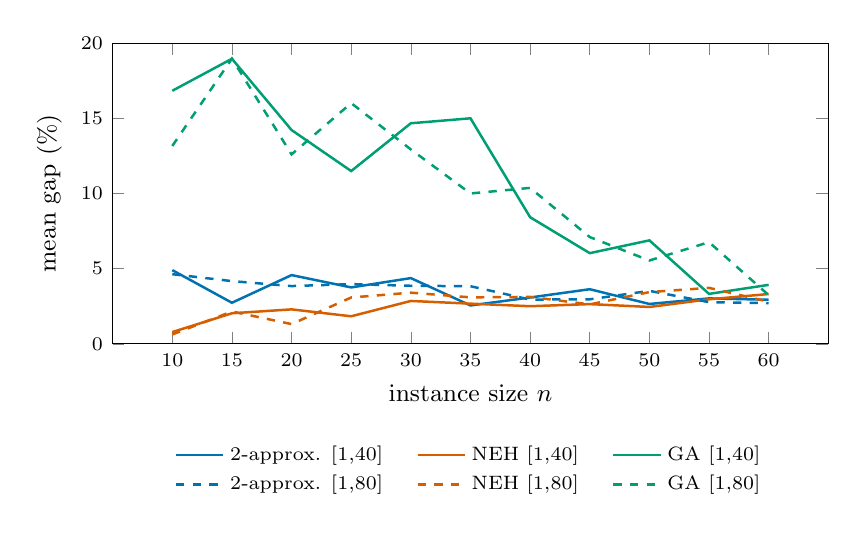
\begin{tikzpicture}
  \begin{axis}[
      width=0.88\textwidth, height=5.4cm,
      xlabel={instance size $n$}, ylabel={mean gap (\%)},
      xtick={10,15,20,25,30,35,40,45,50,55,60}, xticklabels={10,15,20,25,30,35,40,45,50,55,60},
      ymin=0, ymax=20,
      tick label style={font=\scriptsize}, label style={font=\small},
      every axis plot/.append style={line width=0.9pt},
      legend columns=3,
      legend style={font=\scriptsize, at={(0.5,-0.30)}, anchor=north, draw=none,
        /tikz/every even column/.append style={column sep=10pt}},
      ]
      \addplot[apxblue] coordinates {(10,4.90) (15,2.73) (20,4.57) (25,3.75) (30,4.37) (35,2.55) (40,3.08) (45,3.63) (50,2.65) (55,3.02) (60,2.93)};
        \addlegendentry{2-approx. $[1{,}40]$}
      \addplot[nehred] coordinates {(10,0.78) (15,2.03) (20,2.29) (25,1.83) (30,2.85) (35,2.67) (40,2.50) (45,2.64) (50,2.45) (55,2.96) (60,3.31)};
        \addlegendentry{NEH $[1{,}40]$}
      \addplot[gagreen] coordinates {(10,16.83) (15,18.96) (20,14.22) (25,11.49) (30,14.67) (35,15.00) (40,8.42) (45,6.03) (50,6.88) (55,3.32) (60,3.92)};
        \addlegendentry{GA $[1{,}40]$}
      \addplot[apxblue, dashed] coordinates {(10,4.63) (15,4.17) (20,3.84) (25,3.97) (30,3.86) (35,3.83) (40,2.94) (45,2.96) (50,3.52) (55,2.77) (60,2.71)};
        \addlegendentry{2-approx. $[1{,}80]$}
      \addplot[nehred, dashed] coordinates {(10,0.62) (15,2.15) (20,1.31) (25,3.08) (30,3.40) (35,3.09) (40,3.12) (45,2.62) (50,3.44) (55,3.72) (60,2.80)};
        \addlegendentry{NEH $[1{,}80]$}
      \addplot[gagreen, dashed] coordinates {(10,13.16) (15,18.97) (20,12.60) (25,16.01) (30,12.93) (35,10.00) (40,10.37) (45,7.10) (50,5.54) (55,6.76) (60,3.24)};
        \addlegendentry{GA $[1{,}80]$}
  \end{axis}
\end{tikzpicture}
\caption{Mean relative gap of the three heuristics on the small scale, against the optimum the model returned. A solid line is $a_j,b_j\in[1,40]$, a dashed line $a_j,b_j\in[1,80]$.}
\label{fig:gap-small}
\end{figure}

On this scale the three methods end within a point of one another, the search having travelled the
whole way to join the two rules. What still separates them is the price: the model is exact but
close to the limit of its budget, NEH is the closer of the two rules at the bottom of the scale
and the 2-approximation at the top, and the search pays three orders of magnitude above both
rules for a gap of the same order. What that price buys is read on the large scale.

\subsection{The large scale}

On the large scale the three methods separate for good. The rules are flat: the 2-approximation
is the closest on average at $1.81$ per cent over the $32$ configurations, its mean never above
$3.20$ per cent and its worst instance $7.57$ per cent away, and NEH is the furthest at $4.40$
per cent, its gap hardly moving over the scale -- $5.02$ at a hundred jobs against $3.60$ at four
hundred on $[1,40]$, and $5.39$ against $4.47$ on $[1,80]$, with a worst instance $12.64$ per
cent away. The genetic algorithm is the only method whose gap falls as the instance grows, and it
falls steeply: $10.88$ per cent at a hundred and eighty jobs, $5.49$ at two hundred, $2.09$ at
two hundred and forty and $0.22$ at four hundred on $[1,40]$, and $6.99$, $6.34$, $2.09$ and
$0.13$ per cent on $[1,80]$. It passes NEH at $240$ jobs and the 2-approximation at about $260$
on $[1,80]$ and $280$ on $[1,40]$, and over the $640$ instances of the scale it attains the best
value on $318$ of them, against $283$ for the 2-approximation and $42$ for NEH. What it costs is
time and the bottom of the scale: $70.8$\,s an instance on average, against $0.076$\,ms for the
2-approximation and $0.76$\,s for NEH, with $313.5$\,s on its slowest instance of the $600$\,s a
run allows, and its worst configuration and its worst instance both at the bottom, at $10.88$ and
$28.17$ per cent.

The two ranges agree on the ordering of the two rules and disagree on the search. The
2-approximation is closer on the wider range, $1.70$ per cent against $1.92$, and NEH further from
it, $4.79$ against $4.02$, so that the 2-approximation leads NEH on both ranges while the search
overtakes it on one: $4.28$ against $4.02$ per cent on $[1,40]$, where the two are within a quarter
of a point of one another, and $3.65$ against $4.79$ on $[1,80]$.
\Crefrange{tab:results-large-40}{tab:results-large-80} give the two ranges in full, and
\Cref{fig:gap-large} the course of the gap over the scale.

\begin{table}[H]
\resultstable
\caption{The large scale, $a_j,b_j\in[1,40]$: 2-approx., NEH, GA}
\label{tab:results-large-40}
\begin{tabular*}{\resultstabwidth}{@{\extracolsep{\fill}}l r r @{\hspace{14pt}} r r @{\hspace{14pt}} r r@{}}
\toprule
\multirow{2}{*}{$n$} & \multicolumn{2}{c}{2-approx.} & \multicolumn{2}{c}{NEH} & \multicolumn{2}{c}{GA} \\
\cmidrule(lr){2-3}\cmidrule(lr){4-5}\cmidrule(lr){6-7}
 & gap & time (ms) & gap & time (ms) & gap & time (ms) \\
\midrule
$100$ & $\mathbf{3.2}$ $7.6$ & $3.0\mathrm{e}{-2}$ $7.0\mathrm{e}{-2}$ & $5.0$ $7.7$ & $3.5\mathrm{e}1$ $3.6\mathrm{e}1$ & $10.6$ $28.2$ & $1.4\mathrm{e}3$ $1.4\mathrm{e}3$ \\
$120$ & $\mathbf{2.9}$ $5.1$ & $3.0\mathrm{e}{-2}$ $5.0\mathrm{e}{-2}$ & $4.3$ $11.0$ & $6.1\mathrm{e}1$ $6.7\mathrm{e}1$ & $9.7$ $21.4$ & $2.2\mathrm{e}3$ $2.3\mathrm{e}3$ \\
$140$ & $\mathbf{2.7}$ $6.1$ & $3.0\mathrm{e}{-2}$ $4.0\mathrm{e}{-2}$ & $4.1$ $6.2$ & $9.2\mathrm{e}1$ $9.7\mathrm{e}1$ & $10.8$ $23.2$ & $3.2\mathrm{e}3$ $3.3\mathrm{e}3$ \\
$160$ & $\mathbf{1.9}$ $3.7$ & $4.0\mathrm{e}{-2}$ $4.0\mathrm{e}{-2}$ & $4.6$ $7.1$ & $1.3\mathrm{e}2$ $1.4\mathrm{e}2$ & $9.6$ $20.5$ & $4.6\mathrm{e}3$ $4.7\mathrm{e}3$ \\
$180$ & $\mathbf{2.4}$ $5.3$ & $4.0\mathrm{e}{-2}$ $7.0\mathrm{e}{-2}$ & $4.1$ $7.3$ & $1.9\mathrm{e}2$ $2.0\mathrm{e}2$ & $10.9$ $20.4$ & $6.4\mathrm{e}3$ $6.6\mathrm{e}3$ \\
$200$ & $\mathbf{2.1}$ $5.1$ & $5.0\mathrm{e}{-2}$ $6.0\mathrm{e}{-2}$ & $3.9$ $8.5$ & $2.6\mathrm{e}2$ $2.7\mathrm{e}2$ & $5.5$ $14.2$ & $1.1\mathrm{e}4$ $1.1\mathrm{e}4$ \\
$220$ & $\mathbf{2.0}$ $5.1$ & $6.0\mathrm{e}{-2}$ $1.0\mathrm{e}{-1}$ & $3.9$ $5.9$ & $3.5\mathrm{e}2$ $3.5\mathrm{e}2$ & $4.3$ $10.8$ & $1.7\mathrm{e}4$ $1.8\mathrm{e}4$ \\
$240$ & $\mathbf{1.7}$ $3.5$ & $6.0\mathrm{e}{-2}$ $1.0\mathrm{e}{-1}$ & $4.2$ $7.2$ & $4.5\mathrm{e}2$ $4.6\mathrm{e}2$ & $2.1$ $8.1$ & $2.6\mathrm{e}4$ $2.7\mathrm{e}4$ \\
$260$ & $\mathbf{1.7}$ $3.9$ & $7.0\mathrm{e}{-2}$ $8.0\mathrm{e}{-2}$ & $4.0$ $6.7$ & $5.7\mathrm{e}2$ $5.8\mathrm{e}2$ & $1.7$ $6.0$ & $3.9\mathrm{e}4$ $4.0\mathrm{e}4$ \\
$280$ & $1.6$ $4.6$ & $7.0\mathrm{e}{-2}$ $8.0\mathrm{e}{-2}$ & $4.0$ $7.3$ & $7.2\mathrm{e}2$ $7.4\mathrm{e}2$ & $\mathbf{0.8}$ $3.8$ & $5.8\mathrm{e}4$ $5.9\mathrm{e}4$ \\
$300$ & $2.1$ $5.4$ & $8.0\mathrm{e}{-2}$ $1.1\mathrm{e}{-1}$ & $4.1$ $6.2$ & $8.9\mathrm{e}2$ $9.1\mathrm{e}2$ & $\mathbf{0.7}$ $2.0$ & $7.7\mathrm{e}4$ $7.9\mathrm{e}4$ \\
$320$ & $1.4$ $2.7$ & $9.0\mathrm{e}{-2}$ $1.4\mathrm{e}{-1}$ & $3.6$ $6.1$ & $1.1\mathrm{e}3$ $1.1\mathrm{e}3$ & $\mathbf{0.6}$ $2.4$ & $1.0\mathrm{e}5$ $1.0\mathrm{e}5$ \\
$340$ & $1.3$ $4.0$ & $1.0\mathrm{e}{-1}$ $1.5\mathrm{e}{-1}$ & $3.5$ $5.5$ & $1.3\mathrm{e}3$ $1.3\mathrm{e}3$ & $\mathbf{0.4}$ $1.9$ & $1.3\mathrm{e}5$ $1.3\mathrm{e}5$ \\
$360$ & $1.2$ $2.9$ & $1.1\mathrm{e}{-1}$ $1.4\mathrm{e}{-1}$ & $3.7$ $7.2$ & $1.6\mathrm{e}3$ $1.6\mathrm{e}3$ & $\mathbf{0.2}$ $0.9$ & $1.6\mathrm{e}5$ $1.6\mathrm{e}5$ \\
$380$ & $1.3$ $3.1$ & $1.2\mathrm{e}{-1}$ $1.5\mathrm{e}{-1}$ & $3.8$ $6.0$ & $1.9\mathrm{e}3$ $2.1\mathrm{e}3$ & $\mathbf{0.4}$ $1.6$ & $2.1\mathrm{e}5$ $2.2\mathrm{e}5$ \\
$400$ & $1.5$ $3.0$ & $2.0\mathrm{e}{-1}$ $8.9\mathrm{e}{-1}$ & $3.6$ $4.9$ & $2.4\mathrm{e}3$ $2.9\mathrm{e}3$ & $\mathbf{0.2}$ $1.1$ & $2.8\mathrm{e}5$ $3.3\mathrm{e}5$ \\
\bottomrule
\end{tabular*}
\end{table}

\begin{table}[H]
\resultstable
\caption{The large scale, $a_j,b_j\in[1,80]$: 2-approx., NEH, GA}
\label{tab:results-large-80}
\begin{tabular*}{\resultstabwidth}{@{\extracolsep{\fill}}l r r @{\hspace{14pt}} r r @{\hspace{14pt}} r r@{}}
\toprule
\multirow{2}{*}{$n$} & \multicolumn{2}{c}{2-approx.} & \multicolumn{2}{c}{NEH} & \multicolumn{2}{c}{GA} \\
\cmidrule(lr){2-3}\cmidrule(lr){4-5}\cmidrule(lr){6-7}
 & gap & time (ms) & gap & time (ms) & gap & time (ms) \\
\midrule
$100$ & $\mathbf{2.8}$ $5.3$ & $3.0\mathrm{e}{-2}$ $5.0\mathrm{e}{-2}$ & $5.4$ $12.6$ & $3.6\mathrm{e}1$ $3.7\mathrm{e}1$ & $9.0$ $23.6$ & $1.4\mathrm{e}3$ $1.5\mathrm{e}3$ \\
$120$ & $\mathbf{2.4}$ $4.7$ & $3.0\mathrm{e}{-2}$ $6.0\mathrm{e}{-2}$ & $4.6$ $6.5$ & $6.0\mathrm{e}1$ $6.6\mathrm{e}1$ & $9.1$ $20.9$ & $2.2\mathrm{e}3$ $2.2\mathrm{e}3$ \\
$140$ & $\mathbf{2.2}$ $6.0$ & $3.0\mathrm{e}{-2}$ $4.0\mathrm{e}{-2}$ & $4.8$ $8.4$ & $9.1\mathrm{e}1$ $9.3\mathrm{e}1$ & $7.2$ $15.1$ & $3.1\mathrm{e}3$ $3.2\mathrm{e}3$ \\
$160$ & $\mathbf{2.6}$ $5.5$ & $4.0\mathrm{e}{-2}$ $4.0\mathrm{e}{-2}$ & $4.0$ $7.5$ & $1.4\mathrm{e}2$ $1.4\mathrm{e}2$ & $10.2$ $21.9$ & $4.6\mathrm{e}3$ $4.7\mathrm{e}3$ \\
$180$ & $\mathbf{2.1}$ $4.7$ & $4.0\mathrm{e}{-2}$ $5.0\mathrm{e}{-2}$ & $4.7$ $7.2$ & $1.9\mathrm{e}2$ $2.0\mathrm{e}2$ & $7.0$ $17.1$ & $6.4\mathrm{e}3$ $6.7\mathrm{e}3$ \\
$200$ & $\mathbf{1.9}$ $6.6$ & $5.0\mathrm{e}{-2}$ $7.0\mathrm{e}{-2}$ & $5.0$ $8.6$ & $2.6\mathrm{e}2$ $2.7\mathrm{e}2$ & $6.3$ $17.5$ & $1.1\mathrm{e}4$ $1.1\mathrm{e}4$ \\
$220$ & $\mathbf{1.4}$ $3.0$ & $5.0\mathrm{e}{-2}$ $6.0\mathrm{e}{-2}$ & $5.1$ $7.6$ & $3.4\mathrm{e}2$ $3.5\mathrm{e}2$ & $2.5$ $7.3$ & $1.7\mathrm{e}4$ $1.8\mathrm{e}4$ \\
$240$ & $\mathbf{1.3}$ $2.4$ & $6.0\mathrm{e}{-2}$ $7.0\mathrm{e}{-2}$ & $4.6$ $8.0$ & $4.5\mathrm{e}2$ $4.6\mathrm{e}2$ & $2.1$ $6.8$ & $2.6\mathrm{e}4$ $2.7\mathrm{e}4$ \\
$260$ & $1.9$ $4.9$ & $7.0\mathrm{e}{-2}$ $8.0\mathrm{e}{-2}$ & $5.6$ $8.0$ & $5.7\mathrm{e}2$ $5.8\mathrm{e}2$ & $\mathbf{1.9}$ $5.7$ & $3.9\mathrm{e}4$ $4.0\mathrm{e}4$ \\
$280$ & $1.4$ $3.1$ & $7.0\mathrm{e}{-2}$ $9.0\mathrm{e}{-2}$ & $3.9$ $6.5$ & $7.2\mathrm{e}2$ $7.3\mathrm{e}2$ & $\mathbf{0.7}$ $2.4$ & $5.8\mathrm{e}4$ $5.9\mathrm{e}4$ \\
$300$ & $1.2$ $2.9$ & $9.0\mathrm{e}{-2}$ $1.3\mathrm{e}{-1}$ & $4.9$ $6.7$ & $8.9\mathrm{e}2$ $9.1\mathrm{e}2$ & $\mathbf{1.1}$ $3.8$ & $7.7\mathrm{e}4$ $7.8\mathrm{e}4$ \\
$320$ & $1.2$ $3.1$ & $9.0\mathrm{e}{-2}$ $1.2\mathrm{e}{-1}$ & $4.3$ $6.0$ & $1.1\mathrm{e}3$ $1.1\mathrm{e}3$ & $\mathbf{0.5}$ $1.8$ & $9.9\mathrm{e}4$ $1.0\mathrm{e}5$ \\
$340$ & $1.1$ $3.0$ & $1.0\mathrm{e}{-1}$ $1.2\mathrm{e}{-1}$ & $4.6$ $6.6$ & $1.3\mathrm{e}3$ $1.3\mathrm{e}3$ & $\mathbf{0.2}$ $1.0$ & $1.3\mathrm{e}5$ $1.3\mathrm{e}5$ \\
$360$ & $1.2$ $2.2$ & $1.1\mathrm{e}{-1}$ $1.3\mathrm{e}{-1}$ & $5.4$ $6.8$ & $1.6\mathrm{e}3$ $1.6\mathrm{e}3$ & $\mathbf{0.2}$ $1.4$ & $1.6\mathrm{e}5$ $1.6\mathrm{e}5$ \\
$380$ & $1.6$ $3.3$ & $1.2\mathrm{e}{-1}$ $1.3\mathrm{e}{-1}$ & $5.2$ $7.3$ & $1.9\mathrm{e}3$ $2.0\mathrm{e}3$ & $\mathbf{0.4}$ $1.8$ & $2.1\mathrm{e}5$ $2.1\mathrm{e}5$ \\
$400$ & $1.1$ $3.7$ & $2.0\mathrm{e}{-1}$ $4.3\mathrm{e}{-1}$ & $4.5$ $7.7$ & $2.7\mathrm{e}3$ $3.2\mathrm{e}3$ & $\mathbf{0.1}$ $0.7$ & $3.1\mathrm{e}5$ $3.5\mathrm{e}5$ \\
\bottomrule
\end{tabular*}
\end{table}

\begin{figure}[H]
\centering
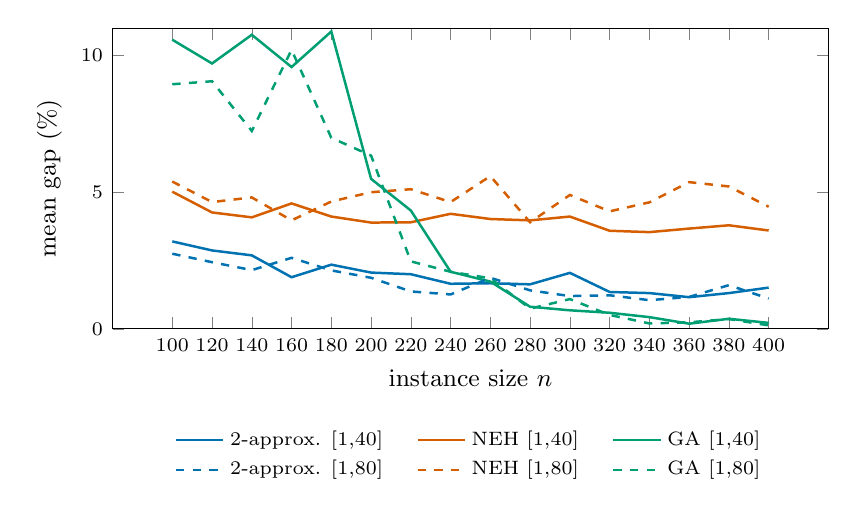
\begin{tikzpicture}
  \begin{axis}[
      width=0.88\textwidth, height=5.4cm,
      xlabel={instance size $n$}, ylabel={mean gap (\%)},
      xtick={100,120,140,160,180,200,220,240,260,280,300,320,340,360,380,400}, xticklabels={100,120,140,160,180,200,220,240,260,280,300,320,340,360,380,400},
      ymin=0, ymax=11,
      tick label style={font=\scriptsize}, label style={font=\small},
      every axis plot/.append style={line width=0.9pt},
      legend columns=3,
      legend style={font=\scriptsize, at={(0.5,-0.30)}, anchor=north, draw=none,
        /tikz/every even column/.append style={column sep=10pt}},
      ]
      \addplot[apxblue] coordinates {(100,3.20) (120,2.87) (140,2.69) (160,1.89) (180,2.35) (200,2.06) (220,2.00) (240,1.65) (260,1.67) (280,1.63) (300,2.05) (320,1.35) (340,1.31) (360,1.16) (380,1.31) (400,1.51)};
        \addlegendentry{2-approx. $[1{,}40]$}
      \addplot[nehred] coordinates {(100,5.02) (120,4.26) (140,4.08) (160,4.59) (180,4.11) (200,3.89) (220,3.90) (240,4.21) (260,4.02) (280,3.97) (300,4.11) (320,3.59) (340,3.54) (360,3.67) (380,3.79) (400,3.60)};
        \addlegendentry{NEH $[1{,}40]$}
      \addplot[gagreen] coordinates {(100,10.58) (120,9.71) (140,10.76) (160,9.58) (180,10.88) (200,5.49) (220,4.33) (240,2.09) (260,1.73) (280,0.81) (300,0.68) (320,0.59) (340,0.43) (360,0.19) (380,0.37) (400,0.22)};
        \addlegendentry{GA $[1{,}40]$}
      \addplot[apxblue, dashed] coordinates {(100,2.75) (120,2.44) (140,2.15) (160,2.60) (180,2.14) (200,1.87) (220,1.37) (240,1.26) (260,1.87) (280,1.41) (300,1.20) (320,1.23) (340,1.05) (360,1.17) (380,1.60) (400,1.11)};
        \addlegendentry{2-approx. $[1{,}80]$}
      \addplot[nehred, dashed] coordinates {(100,5.39) (120,4.64) (140,4.81) (160,3.97) (180,4.66) (200,5.00) (220,5.11) (240,4.64) (260,5.59) (280,3.90) (300,4.90) (320,4.30) (340,4.63) (360,5.37) (380,5.21) (400,4.47)};
        \addlegendentry{NEH $[1{,}80]$}
      \addplot[gagreen, dashed] coordinates {(100,8.95) (120,9.06) (140,7.24) (160,10.21) (180,6.99) (200,6.34) (220,2.47) (240,2.09) (260,1.85) (280,0.74) (300,1.09) (320,0.51) (340,0.20) (360,0.24) (380,0.36) (400,0.13)};
        \addlegendentry{GA $[1{,}80]$}
  \end{axis}
\end{tikzpicture}
\caption{Mean relative gap of the three heuristics on the large scale, against the lower bound $LB$. A solid line is $a_j,b_j\in[1,40]$, a dashed line $a_j,b_j\in[1,80]$.}
\label{fig:gap-large}
\end{figure}

At this scale, then, the rules stay within a few points of the bound while the search falls
through both, and it is there, and only there, that the population buys a value the rules do not
reach. What the study reads is a division of labour rather than a ranking. The
2-approximation is the cheapest method by six orders of magnitude and stays within five per cent
of the optimum on the small scale and within $1.81$ per cent of $LB$ on the large one, which says
that the factor of two of \Cref{thm:approx2} is loose by an order of magnitude on instances of
this kind. What it cannot do is read anything but the weights, and that is the ground NEH takes:
NEH reads the two processing times and no weight, which makes it the closest method at the bottom
of the small scale and the furthest at the top of the large one, where its gap does not close as
the instance grows.

The two methods that carry the study beyond a rule sit at opposite ends of it. The dynamic program
is the only one that certifies an optimum, and it does so cheaply where it applies, at $1.47$\,s
for forty jobs on $[1,40]$, but its applicability is the restriction: two weight classes, at most
a hundred jobs, and a third class that exhausts the memory of the machine before the search
starts. The genetic algorithm is the reverse. It certifies nothing, it costs three orders of
magnitude more than the rules on the small scale and more than ninety times NEH on the large one,
and it is nevertheless the only method that beats both rules, on $318$ of the $640$ large
instances and from about $260$ jobs on. Neither is read on the instances of the other, the dynamic
program on a set of its own at $K=2$ and the search on instances that carry up to thirty weight
classes, so what separates them is not a common benchmark but the question each answers: whether
the optimum can be certified at all, or whether a schedule that beats every rule can be built at
the sizes that arise. The reason the search needs the room is the start it is given: Johnson's
rule carries no weight, so its early generations are spent building the criterion into the
schedule before it can profit from it.

Two properties of the comparison are worth keeping in view. The large-scale gaps are distances to
$LB$, which caps the optimum by the three prefix bounds of \cref{eq:lb} and is tight only where
the heaviest jobs are also the earliest ones; what they order reliably is therefore the methods
and not their absolute quality. And the answers depend on the processing-time range: the average
advantage of the search over NEH, $3.97$ against $4.40$ per cent, is earned on $[1,80]$ alone.

What would extend the study follows from each of its limits. On the exact side the dynamic program
is stopped by memory, so dominance rules that drop a state another state beats, or a solution of
one weight class at a time, are the way past $K=2$, with the scheme of \Cref{sub:fptas} the
memory-lean alternative where they are not enough. On the side of the search, seeding the
population with the order the 2-approximation returns costs microseconds and carries the weights
the Johnson order lacks, which is the cheap way to move the size at which the search overtakes the
rules. Both point at the same economy, of spending the budget where the criterion still moves.

\FloatBarrier
\clearpage

\section{Conclusion}
\label{sec:conclusion}

This paper has shown that the two-machine flow shop with the maximum weighted completion time as
its criterion is strongly NP-hard, and that it admits a structure on which exact computation
becomes possible: an optimal schedule is a permutation, it splits into one block per distinct
weight, Johnson's order holds inside a block, and the blocks follow the weights in non-increasing
order. The dynamic program built on that structure prunes dominated states and runs in
$O(nKV^{3K-3})$ time, the 2-approximation reads the weights alone and runs in $O(n\log n)$ time,
the approximation scheme attains a $(1+\varepsilon)$ guarantee for a constant number of weights,
and the two heuristics, an adapted NEH and a genetic algorithm, cover the sizes at which none of
the exact methods reaches.

The computational study places each of them in its range. The mixed integer model settles all
$440$ small instances to optimality, and at $K=2$ the dynamic program certifies the optimum up to a
hundred jobs on $[1,40]$ and to eighty on $[1,80]$, where it is the $600$\,s limit and not its
correctness that stops it. Against the optimum the 2-approximation stays within $3.5$ per cent on
average and NEH within $2.5$; against the lower bound on the large scale the same two rules stay
within $1.8$ and $4.4$ per cent, while the genetic algorithm, the weakest of the three on small
instances, is the only method whose gap falls as the instance grows, and it passes both rules
beyond about $260$ jobs. The practical reading is a division of labour rather than a ranking: the
rules are cheap and dependable, the exact methods certify within their reach, and the search buys
values that neither rule reaches.

Three extensions follow from the limits of the study, one for each of its methods. The first
concerns the number of machines: the mixed integer formulation of \Cref{sec:preliminaries} is
written for two machines and generalises, the assignment constraints and the completion-time
recursions carrying over to $m>2$ machines with one sequence per machine in place of the single
permutation, since the permutation property that holds for two machines fails in general with
three or more. What the extension costs is size, a set of sequencing variables for every machine,
and not principle.

The second concerns the number of weight classes. The dynamic program is stopped at $K=3$ by its
state space, bounded by $2^{K}V^{3K-3}$, which exhausts the memory of the machine before the search
starts. Branch and bound is the natural successor there, and two of its ingredients are already in
the paper: the block structure gives the branching rule, over the order of the blocks and over the
jobs within one, and the three thresholds $LB_1$, $LB_2$ and $LB_3$ of \Cref{sub:approx2} give a
bound at every node. What such a procedure would keep is part of the certification the program
gives at $K=2$, on instances the program cannot reach.

The third concerns the setting. Both heuristics read only the processing times and the weights, so
they carry over to the distributed flow shop, where several identical flow shops process the jobs
and the assignment of a job to a shop is added to the sequencing decision: the insertion test of
NEH can be taken shop by shop, and the chromosome of the genetic algorithm can carry the assignment
beside the permutation. Variants that keep a two-machine shop inside a larger problem admit the
same treatment. Each of the three moves extends the reach of a method without changing the
structure it exploits.

\bibliographystyle{apalike}
\bibliography{ref_IJPR}

\end{sloppypar}
\end{document}

